% UG project example file, February 2022
%   A minior change in citation, September 2023 [HS]
% Do not change the first two lines of code, except you may delete "logo," if causing problems.
% Understand any problems and seek approval before assuming it's ok to remove ugcheck.
\documentclass[logo,bsc,singlespacing,parskip]{infthesis}
\usepackage{ugcheck}
\usepackage{xcolor}  % Package for colors
\usepackage{listings}
\usepackage{comment}
\usepackage{amsmath}
\usepackage[most]{tcolorbox}
\usepackage{tabularx} % Include this in the preamble
\usepackage{float}
\usepackage{longtable}
\usepackage{hyperref}


\usepackage{amssymb}
\usepackage{amsmath}
\usepackage{amssymb}
\usepackage{array}

\newcommand{\handlerDef}[2]{
    \[
    \text{  #1 := handler} 
      \left\{
    \begin{aligned}
        #2
    \end{aligned}
    \right\}
    \]
}

\newcommand{\effectDef}[2]{
    \[
    \text{#1} \overset{\text{def}}{=} 
    \left\{
    \begin{aligned}
        #2
    \end{aligned}
    \right\}
    \]
}

\newcommand{\operation}[4]{
    #1\left(#2\right)\left(#3. #4\right)
}

\newcommand{\equivalenceStatement}[4]{
\[
\begin{array}{rcl}
\text{\textbf{with} } #1 \text{ \textbf{handle}} & \equiv & \text{\textbf{with} } #3 \text{ \textbf{handle}} \\
\quad \text{#2} & & \quad \text{#4}
\end{array}
\]
}



\newcommand{\with}{
\textbf{with}
}


\newcommand{\effectAndHandlerDef}[2]{
\noindent\begin{tabular}{@{}l@{\hspace{1cm}}l@{}}
\textbf{Effect Definition} & \textbf{Handler Definition} \\
\multicolumn{1}{@{}p{0.45\linewidth}}{\raggedright\vspace*{\fill} #1} & 
\multicolumn{1}{p{0.45\linewidth}}{\raggedright\vspace*{\fill} #2}
\end{tabular}
}

\newcommand{\equivLine}[2]{
\begin{flushleft}
\hspace*{2em} \text{(#1)} \quad $\equiv$ \quad #2
\end{flushleft}
}

\lstdefinelanguage{Koka}{
  keywords={fun, var, match, val, if, then, else, do,  type, struct},
  morekeywords=[2]{return,resume, handle, ctl, with,effect},
  morekeywords=[3]{Sstate, Ready, Blocked, Proc, Nil, Cons, string, int},
  sensitive=true,
  comment=[l]{//},
  morecomment=[s]{/*}{*/},
  morestring=[b]",
}

\lstset{
  language=Koka,
  basicstyle=\scriptsize\ttfamily,
  keywordstyle=\color{purple},          % Group 1: basic syntax
  keywordstyle=[2]\color{blue},         % Group 2: effect-related
  keywordstyle=[3]\color{teal},         % Group 3: data constructors
  commentstyle=\color{green!80!black},
  stringstyle=\color{orange},
  breaklines=true,
  columns=fullflexible,
  showstringspaces=false
}

\tcbset{
  examplebox/.style={
    colback=blue!5!white,
    colframe=blue!75!black,
    boxrule=0.8pt,
    arc=2mm,
    top=1mm,
    bottom=1mm,
    left=1mm,
    right=1mm,
    fonttitle=\bfseries,
    title={Example},
    sharp corners,
    breakable,
    enhanced jigsaw
  }
}



% Include any packages you need below, but don't include any that change the page
% layout or style of the dissertation. By including the ugcheck package above,
% you should catch most accidental changes of page layout though.

\usepackage{microtype} % recommended, but you can remove if it causes problems
\usepackage{cite} % recommended for citations

\begin{document}
\begin{preliminary}

\title{Implementing Unix using Effect Handlers}

\author{Douglas Torrance}

% CHOOSE YOUR DEGREE a):
% please leave just one of the following un-commented
%\course{Artificial Intelligence}
%\course{Artificial Intelligence and Computer Science}
%\course{Artificial Intelligence and Mathematics}
%\course{Artificial Intelligence and Software Engineering}
%\course{Cognitive Science}
\course{Computer Science}
%\course{Computer Science and Management Science}
%\course{Computer Science and Mathematics}
%\course{Computer Science and Physics}
%\course{Software Engineering}
%\course{Master of Informatics} % MInf students

% CHOOSE YOUR DEGREE b):
% please leave just one of the following un-commented
%\project{MInf Project (Part 1) Report}  % 4th year MInf students
%\project{MInf Project (Part 2) Report}  % 5th year MInf students
\project{4th Year Project Report}        % all other UG4 students


\date{\today}

\abstract{

Most imperative programming languages do not provide a structured facility for handling effects, and functional approaches such as Monads lead to poor modularity and composability issues \cite{jones1993composing}. 


Recently, Algebraic effect handlers have emerged as a flexible, first-class mechanism to define and interpret effects dynamically. This approach provides a structured and modular way to reason about computational effects, such as exceptions, state, and concurrency, and is particularly useful in modelling complex control flows, providing an effective method for addressing several of the key challenges involved in implementing a Unix-like system.
 \cite{ritchie1974unix}. 


Unix was first developed in the 1970s at Bell Labs \cite{ritchie1984unix} to provide a new approach to operating system design. Prior to this, operating systems were typically monolithic and hardware specific. Unix was designed to be a small, portable and multi-user operating system, which emphasised simplicity, modularity and composability. Its key innovations were: 

\begin{itemize}
    \item Everything is treated as a file – a unified approach that simplifies interaction with devices, processes, and data. 
    \item Pipes and redirection - enable seamless composition of commands into larger programs.
    \item Simplified interface - offers a minimal set of system calls, ensuring a consistent approach to process management, file handling, and I/O.
\end{itemize}

This dissertation consists of two parts. In the first part I implement the "Tiny Unix" system described in Hillerström’s \textit{Foundations for Programming and Implementing Effect Handlers} \cite{hillerstrom_foundations_nodate}. Written in the Koka programming language, this implementation provides a modular and composable approach to Unix functionality. 

In the second part, I apply algebraic equivalence rules from Pretnar’s \textit{An Introduction to Algebraic Effects and Handlers} \cite{pretnar_introduction_2015} to analyse the implementation. By leveraging these rules, we can evaluate its properties and compare it to standard Unix implementations. Since certain algebraic standard effects have associated equational theories, we are also able to verify that our implementation adheres to these theoretical foundations.
}

\maketitle

\newenvironment{ethics}
   {\begin{frontenv}{Research Ethics Approval}{\LARGE}}
   {\end{frontenv}\newpage}

\begin{ethics}
This project was planned in accordance with the Informatics Research
Ethics policy. It did not involve any aspects that required approval
from the Informatics Research Ethics committee.

\standarddeclaration
\end{ethics}


\begin{acknowledgements}
I would like to express my sincere thanks to Dr. Sam Lindley for his helpful suggestions, insightful feedback, and valuable input throughout the development of this dissertation. His guidance has been greatly appreciated. I would also like to thank Jesse Sigal for his support and for generously sharing his knowledge and time, which were both immensely helpful during my research.
\end{acknowledgements}


\tableofcontents
\end{preliminary}


\chapter{Introduction}
\section{Motivation}
Effect handlers are increasingly being explored as a way to manage computational effects in programming. Unix provides a useful model for exploring their application, as its abstract system calls serve as an interface for programs to interact with the OS, similarly to how effects provide an interface for programs to cause side effects. 

In this project, we implement these system calls using effect handlers, representing each as an algebraic effect to achieve a concise and modular design. Effect handlers offer a simple and principled way to model Unix’s complex state and control flow challenges, while also enabling formal reasoning about our solutions. I will demonstrate how effect handlers support composable implementations and enhance our ability to reason about intricate control flows, one of their key advantages.
Key motivations and observations include:
\begin{itemize}
    \item \textcolor{red}{Unix’s abstract system calls resemble the concept of effect handlers, in that both represent abstract effectful operations whose implementations can vary depending on context.}
    \item \textcolor{red}{Modelling Unix introduces complex control and scoping issues, which can be handled more naturally in effect-oriented languages compared to imperative approaches. }
\end{itemize}


\section{Aims}
This dissertation aims to:
\begin{itemize}
    \item Outline the theory behind effect handler-oriented programming and provide relevant background on the Unix system, explaining the suitability in using effect handlers to model Unix.
    \item Implement the "Tiny Unix" system in Koka as described in Hillerström's thesis \cite{hillerstrom_foundations_nodate}.
    \item Apply algebraic reasoning techniques to verify that our implementation meets the required Unix specifications. 
    \item Reflect on the effectiveness of using these formal techniques.
    
\end{itemize}

\section{Outline}

\textbf{Chapter 2} introduces the background and research surrounding effect handlers. It provides a brief overview of the Unix system and explains why it serves as an interesting model to implement using effect handlers. The chapter also explores how effects give rise to computational trees, enabling modular reasoning about code.

\textbf{Chapter 3} outlines the implementation of the "Tiny Unix" system, as described abstractly in Hillerström's PhD thesis, using the Koka language. It discusses the advantages of modelling certain control flow and scoping issues with effect handlers, as well as the challenges encountered during implementation.

\textbf{Chapter 4} focuses on reasoning about the “Tiny Unix” implementation. It examines attempts to verify the correctness of features such as environment variables, the file system, nondeterminism, and process synchronisation using algebraic reasoning techniques.

\textbf{Chapter 5} presents the conclusions drawn from this project. It reflects on the difficulties of reasoning formally about effectful programs, the lessons learned, and suggests areas where these reasoning techniques might be more effectively applied in future work.


\chapter{Background}

\section{Algebraic Effects}

Algebraic effects \cite{plotkin_handling_2013} and their handlers \cite{pretnar_introduction_2015} provide a structured approach to managing computational side effects, explicitly denoting effectful computations and handling them non-locally.

Algebraic effects are handled by \textit{effect handlers}, which provide an interpretation for these effects.

\subsection{Effect Signatures}
In an algebraic effect system, effects are described by signatures, which define a collection of named operations that the effect supports. Each operation has a type signature that specifies the arguments it takes and the type of result it returns.

Take the classic example \texttt{State}. This effect models mutable state, and its signature typically includes two operations:
\begin{itemize}
    \item \texttt{Read(fileName : String) : String}
    \item \texttt{Write(fileName : String, contents : String) : Unit}
\end{itemize}



An effect signature serves as an abstract interface for effectful operations. When a program invokes such an operation, it signals a request, without enforcing how the operation is implemented. The semantics are supplied externally by a handler.

Effects are tracked in the \textit{type system}: any function that performs an effect must either handle it locally or declare it in its type. If unhandled, the effect propagates outward, affecting the type signatures of all enclosing functions until it is eventually interpreted. Unhandled effects bubble up the call stack until they are caught by an appropriate exception handler, in much the same way as unhandled exceptions do.

\subsection{Effect Scoping}
Effect handlers allow us to define multiple different handlers for the same effect, each providing a different interpretation. The way the effect is handled depends on the first relevant effect handler which is in scope. This enables dynamic scoping, where the runtime searches outward through enclosing handler scopes to find the first relevant handler for that effect. As a result, the same operation may be interpreted differently depending on the context in which it is used. This approach enables flexible and modular code, with the same effectful code being reused across contexts with different interpretations supplied by handlers.

\textcolor{red}{This is stronger than traditional abstraction: it's inversion of control, where the interpretation is not just abstracted but externally injected.}

\subsection{Capturing Continuations via Resumptions}
One of the defining features that makes effect handlers particularly powerful is their ability to manipulate resumptions. When an effect operation is handled, the handler receives not only the operation’s arguments but also a continuation, also known as a \textit{resumption}, which represents the rest of the computation still to be executed. The handler may resume the computation one or multiple times, or even discard it entirely. This fine-grained control allows for the expression of advanced control patterns such as backtracking, coroutines, cooperative multitasking, and early exits in a modular and concise way.

\subsection{Benefits to Software Structure}

Effect handler’s separate the core business logic of the program from the implementation details of handling side effects. This separation prevents side-effect handling logic from being scattered throughout the codebase, thereby improving modularity. 

For example, consider logging data accesses in a database. Typically, logging logic would need to be implemented in every data access function, violating the Single Responsibility Principle, which states a class (or module) should have only one reason to change. However, by using an effect handler, you can define a logging effect and centralize all logging logic in one place. This modular approach allows for easy composition of effectful operations. 

In languages like Java, chaining effectful operations can obscure where effects occur and how errors are handled, making it difficult to reason about the interactions between operations. Effect handlers address this issue, making them particularly useful for implementing side effects such as asynchronous operations, state management, logging, and exception handling. 

\subsection{Comparison to other Functional Approaches to Side Effects}
In the context of functional programming, effect handlers provide a simple and lightweight method for managing side effects. They serve as a viable alternative to monads, offering a more flexible approach. Unlike monads, which can become rigid once defined, effect handlers allow for greater modification. Additionally, they simplify the combination of multiple side effects, avoiding the complexity of monad transformers. In some cases, effect handlers also offer better performance by eliminating the overhead of repeatedly wrapping and unwrapping values within monadic structures. 


\section{Syntax for Effect Handlers}

\subsection{Effect System}
Effect Handler oriented languages have what is known as an effect system \cite{bauer_effect_2013}. This describes the computational effects that may occur when a piece of code is executed. An effect system is typically an extension of a type system. Effect systems can be used to enforce effect safety, ensuring all effects are handled and functions only perform the side effects denotd in their effect signature



\lstset{
backgroundcolor=\color{gray!5}, % Set background color
    basicstyle=\ttfamily,              % Use monospace font
    frame=none,                      % Add a frame around the pseudocode
    numbers=none,                      % No line numbers
    tabsize=4                          % Set tab size
}




\subsection{Effect Type}
An effect type provides an explicit way to denote the side effects that a function performs. Each effect type can have multiple effectful operations. Each effectful operation can have parameters with value types and a valued return type. Note that operations can also produce effects and therefore have effect types.

\begin{lstlisting}
effect exception
    ctl exn(error_msg : string) : a 

fun safe_div (x : int, y: int) : exn int
    if y == 0 then exn("div by zero") else return x/y
\end{lstlisting}

Pure functions use the unit effect type. This shows it has no side effects. 

\begin{lstlisting}
fun add (x: Int, y: int) : () int {
	return x + y
}
\end{lstlisting}

\section{Shallow vs Deep Handlers}
There are two approaches to implementing effect handlers in a effect-oriented language: \textit{Deep handlers} and \textit{Shallow handlers}. These differ in the way that they handle continuations.

A Deep handler \cite{hillerstrom_foundations_nodate}  implicitly reinstalls itself on all of its continuations. This means that when a deep handler is applied, \textbf{all} subsequent effects in its continuations are handled by that same handler. 

By contrast, a Shallow handler \cite{ryu_shallow_2018} only manages the \textbf{first} effect caused by a computation. In this scenario, any resumed continuation is no longer wrapped by the handler, so the programmer must provide an additional handler to handle the further effects the continuations may perform.

Both Deep and Shallow handlers can simulate each other's behaviour \cite{deepAsShallow}. However, it may make more sense to use one over the other in certain contexts. Note, most languages only support one or the other. As of 2025, deep handlers are the more popular choice in effect-oriented languages \cite{}.

\subsection{Effectful Programs as Computational Trees}
Effectful programs can be thought of as forming a \textit{computational tree}, with the finished computations representing the leaves, i.e. pure return values, and the effects representing the nodes. Each node requires an effect handler for interpretation, and each effect handler receives a first class syntactic representation of the continuation, known as a \textit{resumption}. 

Effect handlers allow for branching depending on how they use their continuations. A handler may: 
\begin{itemize}
    \item Return a value without resuming the continuation, producing a leaf. For example, an exception discards the rest of the computation simply returns an error code.
    \item Resume the continuation once forming a single branch. For example, a Read operation returns the retrieved value and continues normal execution from there. 
    \item Resume the continuation multiple times, creating multiple branches. For example a process forking multiple children
\end{itemize}

\textcolor{red}{effectful programs “build a computational tree” of possible operations and returns, and effect handlers “fold” that tree.}


The difference between Shallow and Deep handlers can be illustrated by showing how each evaluates the computational tree differently.

A deep handler is analogous to a fold over a computational tree \cite{hillerstrom_foundations_nodate}. It provides an interpretation for each operation it handles given its leaves and subtrees. Like a fold, a deep handler traverses the entire computation tree, recursively handling both the current operation and each operation within its continuations. This makes deep handlers easy to reason about, as we can assume the way that the continuation will be interpreted will be consistent, giving it an \textit{algebraic structure}.

However, a shallow handler does not recurse like this: it is only applied to the first operation it sees. This means the handler must be explicitly reapplied to its continuations if we are to interpret their subsequent operations. This makes formal reasoning more difficult, but it does provide more flexible control over how effects are handled.

\section{Reasoning}
Continuing on with our analogy of effectful programs as computational trees, we can isolate parts of the tree as self contained sub programs and reason about them independently. 


As Deep handlers correspond to a fold over the entire computation, every effect gets interpreted consistently by the same handling clause. This consistency means that if we prove a certain rewrite law we can apply it anywhere in that computation. 

Certain standard algebraic effects (state, non-determinism, ...) 

\section{Unix}
The first edition of the Unix operating system was released by Bell Labs in 1971 \cite{ritchie1974unix}. Written in the C programming language, it was one of the first systems to prioritise portability across hardware platforms, making it extremely popular and influential \cite{blair1985critique}.

Unix was created to provide a portable, multi-user, multi-tasking system and introduced several fundamental innovations including: a hierarchical file system; a uniform \textit{“everything is a file”} interface; and offered powerful process management through system calls like \textit{fork} and \textit{exec}.  It promoted simplicity, modularity, and composition, principles that distinguished it from the large, monolithic systems of its time and that continue to influence modern operating systems like Linux \cite{gancarz2003linux}.

The “everything is a file” model provides a consistent interface for interacting with system resources. Abstract operations, such as system calls, are interpreted by handlers that act as self-contained modules, assigning specific behaviours for I/O, process control, or scheduling. This modular design reflects the Unix philosophy\cite{raymond2003art} of building systems from small, composable components.

What makes Unix interesting from a control flow perspective is the rich set of mechanisms it provides for suspending, resuming and branching computations\cite{stevens2013advanced}. Process scheduling can exhibit non-linear control flow, allowing computations to split into separate execution paths and forcing them to be paused.

Alongside complex control flow, Unix also introduces subtle scoping challenges. It must be able to support both global and local scoping for state. Processes must have independent access to their own resources and must be able to duplicate their own state for their children \cite{aiken2006deconstructing}. Importantly, the same variable name or identifier may refer to different resources in different processes, enabling compositional abstractions like piping and redirection. They must of course also be able to access global state represented by the file system.

Unix presents exactly the kind of challenges that effect handlers excel at solving: control flow is non-trivial, state is both local and global, and system calls are abstract interfaces that demand interpretation. These features make Unix an ideal case for demonstrating the power of effect handlers, and many papers on effect handlers use Unix features to demonstrate the strengths of the effect handlers.



\section{Evaluating Previous work}
In his 2021 paper \textit{Foundations for Programming and Implementing Effect Handlers} \cite{hillerstrom_foundations_nodate}, Daniel Hillerström implemented a theoretical implementation of Unix. He draws an analogy between operating systems and effect handlers, arguing that both interpret a series of abstract invocations. In the case of the OS, these are system calls; in the case of effect handlers, these are operations. The composition of effect handlers, which he describes as “tiny operating systems”, can provide semantics for a Unix implementation. In this dissertation, I use Koka to create a concrete implementation of the abstract syntax Hillerström used in his paper. I will then use equational theory and algebraic equivalences to show my implementation is correct.

There are several papers which examine reasoning about effect handlers. Pretnar's \textit{The Logic and Handling of Algebraic Effects} \cite{Pretnar:2010} uses algebraic equations to reason about abstract properties of state, exceptions and nondeterminism. McLaughlin's PhD thesis \textit{Relational Reasoning for Effects and Handlers} \cite{McLaughlin2020} uses automated reasoning techniques to verify the correctness of an effect handler implementation for Unix-style pipes. 

However, the most relevant for this dissertation is \textit{Not by equations alone: Reasoning with extensible effects} by Oleg Kiselyov, Shin-Cheng Mu and Amr Sabry \cite{kiselyov2021not}, which outlines the limitations of using equational laws to reason about effectful programs. They show how composition can break down algebraic laws which held in isolation. \textcolor{red}{It suggests stronger notions of congruence, i.e. proving expressions are equivalent under different contexts are required.}



\chapter{Unix Implementation}
Having described the theoretical benefits of effect handlers in the previous chapter, we now show the practical implementation of the "Tiny Unix" system, written by Hillerström, in the Koka programming language. 

The features we implement serve as good examples of problems that are difficult to model in traditional programming paradigms. These include problems concerning dynamic scoping, global state, control flow interruptions, and reasoning about suspended computations.

We will show how Koka allows us to implement each effect independently and then compose them together to express this behaviour cleanly and concisely.
In his thesis, Hillerström uses a pseudo-lambda calculus that can switch between deep and shallow handlers. Koka primarily uses deep handlers, enabling us to implement each effect independently, expressing complex behaviour in a clean and concise manner.



\section{Process Status}
In Unix, processes provide an exit code upon termination. A return code of 0 signifies successful execution, while any non-zero value indicates an error. 

We begin by defining the exit effect, which includes a single exit operation parameterised by an integer:
\begin{lstlisting}
effect exit
  ctl exit(n : int) : a
\end{lstlisting}

\vspace{1em}
We can now write the exit handler. It can be seen that the function's signature expects the parameter action as a paused computation, which produces an exit effect.

\begin{lstlisting}
fun status(action : () -> <exit|e> a) : e int
    with final ctl exit(code) code
        action()
        0
\end{lstlisting}
In Hillerström’s language, it was necessary to introduce an absurd function to coerce the valueless return into a form that made sense within the language’s type system. In contrast, Koka allows us to return a value directly without requiring a resumption. In cases where a function returns without explicitly calling exit(n), we assume it has exited successfully and simply return 0.

\section{Basic IO}
Hillerström first models a simplified form of state. From the effect signature, we can see that writes can be labelled with a file descriptor. However, in our implementation, we defer this functionality until later. Initially, we treat all writes as if they are directed to the same output stream, which we conceptualise as stdout, regardless of the specified file descriptor.

\begin{lstlisting}
effect bio
    fun writeBio( fd : filedesc, s : string ) : ()
\end{lstlisting}
\vspace{1em}
Here we define the handler:

\begin{lstlisting}
fun bio( action : () -> <bio|e> a ) : e (a,string)
  var buf := ""    
  with handler
    return (x) -> (x, buf)
    fun writeBio(fd, s) -> { buf := buf ++ s }
  action()
\end{lstlisting}

Note that, unlike in Hillerström’s implementation, we do not require explicit \lstinline{resume} keywords. In Koka, effects of type \lstinline{fun} perform the effective operation and then continue execution immediately.

\section{Users and Environment Variables}
Environment variables are key-value pairs stored in the environment of a process. In this implementation, provide an example by storing the current user's name as an environment variable.

We define users as a \lstinline{sum} type:
\begin{lstlisting}
type user = Root, Alice, Bob
\end{lstlisting}

We define two effects: \lstinline{su}, which is parameterised by the user to switch to, and \lstinline{whoami()}, which returns the current user as a string.

\begin{lstlisting}
effect su
  ctl su( u : user ) : ()

effect whoami
  fun whoami() : string
\end{lstlisting}


\begin{lstlisting}
fun env( user : user, action : () -> <whoami|e> a ) : e a
  with fun whoami() 
    match user
      Root  -> "root"
      Alice -> "alice"
      Bob   -> "bob"
  action()
\end{lstlisting}

Next, we define separate handlers for the \lstinline{su} and \lstinline{whoami()} effects:
\begin{lstlisting}
fun session-mgr( initial-user : user, action : () -> <su,whoami|e> a ) : e a
  with env(initial-user)
  with ctl su( u : user )
         mask<whoami>
           with env(u)
           resume(())
  action()

fun env( user : user, action : () -> <whoami|e> a ) : e a
  with fun whoami() 
    match user
      Root  -> "root"
      Alice -> "alice"
      Bob   -> "bob"
  action()
\end{lstlisting}

The \lstinline{env} handler is parameterised by the current user, enabling it to handle \lstinline{whoami()} operations by returning this user's identity.

\lstinline{session_mgr} manages user switches by rewrapping the continuation in a new \lstinline{env} handler, parameterised by the new user. This method offers greater modularity compared to global variables because it fully encapsulates state within the effect handler itself. This is an example of dynamic scoping, a technique that will be especially useful in the next section, which deals with process forking.

\section{Multi-Process System}
\subsection{Forking}
A forking operation creates a new computational thread that continues independently from the original. Hillerström describes how forking introduces nondeterminism into a system.  From the perspective of each process in the system, it is unclear which order the processes will execute, as this is managed by the operating system's scheduling policy. 

It will be seen that the fork operation returns boolean:
\begin{lstlisting}
effect fork
  ctl fork() : bool     

\end{lstlisting}

\begin{lstlisting}
fun forking( action : () -> <fork|e> a ) : e list<a>
  with handler
    return(x) [x]
    ctl fork() resume(True) ++ resume(False)
  action()
\end{lstlisting}

It will be seen that the forking handler introduces two resumptions, splitting computation into two paths. The resumption parameterised with \lstinline{True} represents the parent process and the resumption with \lstinline{False} represents the child process. Resumptions are returned as a list which can be used by the scheduler. 

The \lstinline{fork} operation is used in code structures such as:
\vspace{-1em}
\begin{figure}[H]
    \centering
    \begin{lstlisting}
    if fork() {
        // ... parent specific code
    }
    else{
        /// ... child specific code
    }
    \end{lstlisting}
    \caption{Example of control flow branching via \texttt{fork()}, where the parent and child execute different code paths.}
\end{figure}


\subsection{Scheduling}
Forking gives us the capability to spawn new processes, which our handler returns as a list of paused processes. A scheduling algorithm must be implemented to interleave the running of these processes.

We must first differentiate between a process that has finished and one which has just temporarily paused. We introduce a data type, \lstinline{pstate}, to represent these two states.
\begin{lstlisting}
type pstate<e,a>
  Done(result : a)
  Paused(resumption : () -> e pstate<e,a> )
\end{lstlisting}

Currently, there is no way for a process to indicate it is ready to pause; once it has started, it will execute until it finishes. So we introduce an effect called \lstinline{interrupt} and its effect handler \lstinline{reify-process} as a way of yielding control to the scheduler allowing the interleaving of processes.

\begin{lstlisting}
effect interrupt
  ctl interrupt() : ()

fun reify-process(action : () -> <interrupt|e> a) : e pstate<e,a> 
  with handler  
    return(x) -> Done(x)
    ctl interrupt() -> Paused(fn() resume(()))
  action()
\end{lstlisting}
A co-operative concurrency model has been implemented, meaning that interrupts must be done manually by the programmer. Finally, a scheduler is introduced to coordinate the running of the processes: 
\begin{lstlisting}
fun scheduler( pstates : list<pstate<<fork,div|e>,a>> ) : <div|e> list<a>
  fun schedule( paused : list<pstate<<fork,div|e>,a>>, done : list<a> ) : <div|e> list<a>
    match paused
      Nil -> done
      Cons(Done(x),ps') -> schedule(ps', Cons(x,done))
      Cons(Paused(m),ps') ->
        val ps = forking( m )
        schedule( ps' ++ ps, done )
  schedule(pstates,[])

fun timeshare( action : () -> <fork,interrupt,div|e> a ) : <div|e> list<a>
  val p = Paused( fn() reify-process(action) )
  scheduler([p])
\end{lstlisting}
This scheduler maintains two lists of processes; one containing paused processes, the other containing finished processes, and works recursively. It runs the first process in the paused list until it reaches an interrupt. It then runs the scheduler again, with this process added to the end of the paused queue. When a process finishes, it is added to the \lstinline{done} queue. This procedure is then repeated until there are no processes left in the \lstinline{paused} queue.

\section{Serial File System}
In this section, we implement a more realistic version of the file system implemented earlier. A Unix file system is implemented on top of an array of bytes. Unix structures this medium into the following key regions to facilitate file management:
\begin{itemize}
    \item The \textit{Directory Region} - this stores mappings between human-readable filenames and their corresponding Inode indexes.
    \item The \textit{Inode Region} - the Inode list contains meta data about each file.
    \item The \textit{Data Region} - this stores the actual contents of file which are accessed via pointers stored in the INode.
\end{itemize}

The file system is defined as a record type, composed of the above three lists and two integers to point where the next free inode and data regions are located.

\begin{lstlisting}
type directory 
  Directory
    d_list : list<(string, int)>

type dataRegion 
  DataRegion
    dr : list<(int, string)>

type iNode
  INode
    no : int
    loc : int

type iList 
  IList
    il : list<(int, iNode)> 

struct fileSystem
  dir   : directory
  ilist : iList
  dreg  : dataRegion
  dnext : int
  inext : int

\end{lstlisting}

We define the initial file system state \texttt{fs0} as:
\begin{lstlisting}
val fs0 : fileSystem =
  FileSystem (
    Directory([("stdout", 0)]),
    IList([(0, INode ( 1, loc = 0 ))]),
    DataRegion([(0, "")]),
    1,
    1)
\end{lstlisting}

\subsection{File Reading and Writing}

Effects for reading and writing to our file system are then defined. The effect \lstinline{read} is parameterised with an iNode number and returns an \lstinline{Option<String>} type, which indicates the success or failure of a read operation from the specified iNode. The \lstinline{write} operation takes an integer to denote the iNode and a string to append to the file associated with this iNode. It does not indicate whether or not the write succeeded.

\begin{lstlisting}
effect fileRW
    fun read( ino : int ) : option<string>
    fun write( ino : int, s : string ) : ()
\end{lstlisting}



\begin{lstlisting}
fun fread( ino : int, fs : fileSystem ) : <div,fail|e> string
    val inode = lookupINode(ino, fs.ilist)
    val ret = lookupDataRegion(inode.loc, fs.dreg)
    ret
\end{lstlisting}

The various \texttt{lookup} utility functions must account for the possibility that they could fail. We introduce a \texttt{fail} effect and an associated \texttt{withDefault} handler to deal with this scenario.

\begin{lstlisting}
effect fail
  ctl fail() : a

fun withDefault<a>(default: a, m: () -> <div,fail|e>a) : <div|e>a
  with handler
    return(x) -> x
    ctl fail() -> default
  m()
\end{lstlisting}

The  handler for \lstinline{read} and \lstinline{write} operations in our system is shown below. We wrap \lstinline{read} and \lstinline{write} operations with \lstinline{withDefault} to provide error handling and failures in \lstinline{lookup} and \lstinline{modify} functions return \lstinline{None}.


\begin{lstlisting}
fun fileRW<a>(m: () -> <fileRW,div,state<fileSystem>|e>a) : <state<fileSystem>,div|e>  a {
  with handler
    fun read(ino) {
      val cs = withDefault(None, fn() -> Some(fread(ino, get())))
      cs
    }
    fun write(ino, cs) {
      withDefault((), fn() {
          val fsys  = get()
          val fsys' = fwrite(ino, cs, fsys)
          put(fsys')
          ()
      })
    }
  m()
}
\end{lstlisting}


\subsection{File Creation and Opening}

The \lstinline{fileCO} effect and operations to create and open files are shown below:

\begin{lstlisting}
effect fileCO
  ctl create( fname : string ) : option<int>
  ctl open( fname : string ) : option<int>
\end{lstlisting}
A simplified serial file system is shown below. Note, the system does not track which processes have opened each file in the Open File Table. Therefore, concurrent reading or writing operations to the same files from multiple processes are not restricted - our \lstinline{open} file operation simply retrieves the associated iNode from the file name in the directory.

\begin{lstlisting}
fun fopen(fname: string, fs : fileSystem) 
    match fs.dir {
        Directory(d_list) ->
        match d_list {
            Nil        -> fail()  
            Cons((k, v), rest) ->
            if k == fname then v
            else lookupDirectory(fname, Directory(rest))
        }
    }
\end{lstlisting}    


When creating a file we must handle two possibilities:
\begin{enumerate}
    \item \textbf{The file already exists.} In this case we must remove the file contents and simply return the associated  iNode and the modified FileSystem.
    \item \textbf{The file doesn't exist.} In this case we must first allocate space in the data region, then allocate an iNode and then add the file name to the directory. Here the operation returns the newly created iNode of this file and the modified FileSystem as a tuple.
\end{enumerate}

\begin{lstlisting}
fun fcreate(fname: string, fs: fileSystem) : <div,fail> (int, fileSystem) 
  if has(fname, fs.dir) then {
    val ino = fopen(fname, fs)  
    val inode = lookupINode(ino, fs.ilist)  
    val dreg' = modifyDataRegion(inode.loc, "", fs.dreg)  

    (ino, FileSystem(fs.dir, fs.ilist, dreg', fs.dnext, fs.inext))  
  }
  else {
    val loc = fs.dnext  // next free data block index
    val dreg' = DataRegion(Cons((loc, ""), fs.dreg.dr))  
    val ino = fs.inext  // next free i-node index
    val inode = INode(loc, 1)  
    val ilist' = IList(Cons((ino, inode) , fs.ilist.il))  
    val dir' = Directory(Cons((fname, ino), fs.dir.d_list))
    
    val fs' = FileSystem(dir', ilist', dreg', fs.dnext + 1, fs.inext + 1)  
    (ino, fs')
  }

fun has<a, b>(key: string, xs: directory) : <div> bool
    withDefault(False, fn() {
        val disc = lookupDirectory(key, xs)  
        True  
    })
\end{lstlisting}

We can now implement the handler for the \lstinline{create} an \lstinline{open} operations.

\begin{lstlisting}
fun fileCreateOpen<a>(action : () -> <fileCO, div, state<fileSystem>|e> a) : <state<fileSystem>,div|e> a
  with handler {
    return(x) -> x
    ctl create(name) {
      val maybeIno = withDefault(None, fn() {
        val fs0 = get()
        val (ino,fs1) = fcreate(name, fs0)
        put(fs1)
        Some(ino)
      })
      resume(maybeIno)
    }

    ctl open(name) {
      val maybeIno = withDefault(None, fn() {
        val fs0 = get()
        val ino = fopen(name, fs0)
        Some(ino)
      })
      resume(maybeIno)}  
  }
  action()
\end{lstlisting}

\subsection{File Linking and Unlinking}
Operations for \textbf{linking} and \textbf{unlinking} files, are shown below. Unix supports two types of linking, \textbf{hard} and \textbf{symbolic}. With hard links, multiple file names point to the same iNode, allowing the creation of multiple references to the same underlying file.

\begin{lstlisting}
effect fileLU
  ctl link(src: string, tgt : string) :()
  ctl unlink(tgt : string) :()
\end{lstlisting}

An example of the linking implementation is shown below:
\begin{lstlisting}
fun flink(src : string, dest : string, fs : fileSystem) : <div,fail> fileSystem {
  if has(dest, fs.dir) then
    fail()  // If `dest` exists, fail
  else {
    val ino = lookupDirectory(src, fs.dir)

    val dir' = Directory(Cons((dest, ino), fs.dir.d_list))

    val inode = lookupINode(ino, fs.ilist)

    val inode' = INode(inode.no, inode.loc + 1)

    val ilist' = modifyINode(ino, inode', fs.ilist)

    FileSystem(dir', ilist', fs.dreg, fs.dnext, fs.inext)
  }
}
\end{lstlisting}


\section{Piping}
Piping is a important core feature of Unix,  as it allows developers to write  small, focused modules rather than monolothic programs. These modules can be composed together to create new functionalities, removing the necessity to write new programs for each new functionality.

The signatures below show the \lstinline{produce} and \lstinline{consume} effects required to implement piping: \lstinline{produce} is parametrised by a value of type \lstinline{b}, allowing it to \textit{yield} a value to the read-end. Conversely, the \lstinline{consume} operation has a return type of \lstinline{b}, indicating that it awaits for a value.
\begin{lstlisting}
effect produce<b>
  ctl produce(x : b) : ()   

effect consume<b>
  ctl consume() : b         

\end{lstlisting}

The shallow handlers, \lstinline{pipe} and \lstinline{copipe}, mutually recurse to handle \lstinline{consume} and \lstinline{produce} operations. In our system this is handled as a function, whereas in Unix, these are implemented as processes which allowing for concurrency.

\begin{lstlisting}
fun pipe<a,b,e>(p : () -> <produce<b>|e> a,c : () -> <consume <b>|e> a) : e a
    with raw ctl consume()
        copipe(fn(x) rcontext.resume-shallow(x), p)
        return(x) -> x

fun copipe(c : b -><consume<b>, div|e>, c : () -> <produce<b>, div|e> a): <div|e> a
    with raw ctl produce(y)
        pipe(fn() rcontext.resume-shallow(()), fn() c(y))
\end{lstlisting}

\section{Process Synchronisation}

In this section we introduce more advanced techniques for process scheduling to allow for partial ordering. 

Currently, our scheduling system does not have any synchronisation primitives, so we have no control over how processes interact. The scheduler can be extended to provide  partial ordering between processes. Controlling the order in which processes are executed, vital when executing tasks that have temporal dependencies. 

We begin by defining the following effects:


\begin{enumerate}
    \item We update the forking mechanism \lstinline{ufork} to a return an integer instead of a boolean. The operation still  returns twice: it returns the process identifier (PID) to the parent, and 0 to the child. 

    \item The \lstinline{interrupt} operation is implemented exactly the same as before, i.e. it is invoked to suspend the current process to allow another to run. 

    \item The \lstinline{wait} operation is parametrised with an integer, which represents the process which must be completed before the invoking process can continue. The invoking process will be blocked until this happens.
\end{enumerate}


\begin{lstlisting}
effect co
  ctl ufork() : int
  ctl wait(pid: int): ()
  ctl sinterrupt() :()
\end{lstlisting}


We then define the following three data types: 

\begin{enumerate}
    \item \lstinline{proc} - represents a reified process, i.e. a process that has been captured in a function which can be run later. It returns a list of type \lstinline{list<int, a>} which represents the \textit{PID} and results of all the processes created during the execution of this process.  

    \item \lstinline{pstate} - represents the internal scheduling state of a single process. It is a \lstinline{sum} type composed of two constructors, \lstinline{Ready} and \lstinline{Blocked}. The latter has an additional field, \textit{PID}, which is the identifier of the process that it is waiting on. 

    \item \lstinline{sstate} - represents the complete state of the scheduler and keeps track of everything it needs to manage and schedule multiple processes i.e. a list the processes still to be executed, the list of completed processes, the id (\lstinline{pid}) of the process currently being executed,  and a fresh process id \lstinline{pnext}.

\end{enumerate}


\begin{lstlisting}
rec type proc<a>
  Proc
    p: sstate<a> -> list<(int, a)>

type spstate<a>
  Ready
    r : proc<a>
  Blocked 
    pid :int 
    proc:proc<a>

type sstate<a> 
  Sstate     
    q : list<(int, spstate<a>)>
    done  : list<(int,a)>
    pid   : int
    pnext : int
\end{lstlisting}


We then define an auxiliary function which abstracts some of the scheduling logic. This function considers three cases:
\begin{enumerate}
    \item \textbf{Ready} - here the next process is run immediately.
    \item \textbf{Blocked} - here the blocked process is sent to the back of the queue.
    \item An Empty queue - here there are no more processes to run, so the list of process results is returned.
\end{enumerate}

\begin{lstlisting}
fun runNext<a>(st: sstate<a> ) : <div,co|e> list<(int,a)> 
  match st.q
    Nil -> st.done
    Cons((bpid, Blocked(pid', proc)), ps) -> 
      val newQ = ps ++ [(bpid, Blocked(pid', proc))]
      val newsState =  Sstate (q = newQ, done = st.done, pid = st.pid, pnext = st.pnext)
      runNext(newsState) 
    Cons((rpid, Ready(proc)), ps) -> 
      val newState =  Sstate (q = ps, done = st.done, pid = rpid, pnext = st.pnext)
      val res = proc.p
      res(newState)
\end{lstlisting}

The scheduler below is a handler for the concurrency effect, \lstinline{co}, that occurs when running the suspended computation, \lstinline{comp}. 


\begin{lstlisting}
fun scheduler<a,e>(comp : () -> <co,div> a, init : sstate<a>) : <div|e> list<(int,a)>
  with handler
    return(x) -> 
      val done'   = Cons((init.pid, x), init.done)
      val newInit = Sstate( q=init.q, done = done', pid = init.pid, pnext= init.pnext)
      runNext(newInit)

    ctl ufork() -> 
      val childProc  = fn(st) ->  resume(0, stChild)  
      val childPid   = init.pnext
      val newQ       =  init.q ++ 
                        [(childPid, Ready(childProc(st)))]
      val st'        = SState (q = newQ, done=init.done, pid=init.pid, pnext = childPid + 1 )
      r(childPid, st')

    ctl sinterrupt() ->
      val interrupted = fn(stInt) -> resume(())
      val newQ        = init.q ++ [(init.pid, Ready(Proc(interrupted)))]
      val _ = runNext(Sstate(q = newQ, done = init.done, pid = init.pid, pnext = init.pnext))
      ()

    ctl wait(pid') ->
      val waitingProc = fn(stWait) -> r((), stWait)
      val newQ =
        if hasPid(pid', init.q)
        then init.q ++ [(init.pid, Blocked(pid', Proc(waitingProc)))]
        else init.q ++ [(init.pid, Ready(Proc(waitingProc)))]
      runNext(Sstate( q = newQ, done = init.done, pid=init.pid,pnext=init.pnext))      
  comp()
\end{lstlisting}    
The scheduler handles \lstinline{fork} operations by constructing a child process in a \lstinline{Ready} state, adding it to the end of the process queue. The child's resumption is parametrised with 0 to indicate to the resumption that it is child process. Finally, we parametrise the resumption to the parent with the \textit{PID} of the child process.

The \lstinline{wait} operation is parametrised by an integer which indicates the process id of the process it is waiting upon. The process queue is checked for the id of the process it is waiting for. If this process is in the queue, the waiting process is added in a Blocked state to the end of the process queue. Otherwise, it is added in a \textit{ready} state to the end of the process queue.

\lstinline{interrupt} simply adds the current process to the end of the process queue.

\section{Chapter Conclusion}

In this chapter we have shown how effect handler-oriented programming provides a clean, modular and composable framework for solving complex control flow and dynamic scoping problems. Using a Unix-like system as a case study, we have demonstrated how features such as \textit{file I/O}, \textit{environment variables}, \textit{process forking}, and \textit{scheduling} can each be modelled as distinct effects and handled independently. 


In the next chapter we will demonstrate how the same modular handler-based abstractions that aid program design also support program reasoning and verification.




\chapter{Reasoning}

In this section we reason about deep handlers using algebraic equivalences, as defined in Pretnar's \textit{Handlers Tutorial} \cite{pretnar_introduction_2015}, (\textit{see figure \ref{fig:equational-laws} below}).  These equivalences provide a method for proving formal properties for  programs implemented using deep effect handlers. Using these rules to transform one computation into another, computations can be shown to be \textit{observationally equivalent}.

In the context of effectful computations, observational equivalence holds when two computations, possibly with different internal structure or steps, result in the same sequence of externally visible effects \cite{sannella1987observational}. In other words, from the perspective of any observer or context interacting with the computation, the computations behave identically, despite any internal differences. External observers include the file system or user IO, i.e. system that could observe or be affected by the computations execution.

\textcolor{red}{Effect handlers make this kind of reasoning possible by separating the syntax and semantics of effects \cite{TheLogicAndHandlingOfAlgebraicEffects}. }

In what follows, I attempt to demonstrate the of use algebraic equivalences to verify the correctness of my Unix implementation. Note, where associated equational theories exist for the effects modelled, such as state or nondeterminism, I show where my implementations satisfy the laws of those theories. In the case where no established equational theory applies, I apply equivalence rules to demonstrate why my implementation behaves as intended.


\begin{figure}[H]
    \centering
    \begin{tcolorbox}[colframe=black, colback=white, sharp corners]
    \begin{align*}
        &\text{(1) } \quad \text{do } x \leftarrow \text{return } v \; \text{in } c \equiv c[v/x] \\
        &\text{(2) } \quad \text{do } x \leftarrow \text{op}(v; y.\, c_1) \; \text{in } c_2 \equiv \text{op}(v; y.\, \text{do } x \leftarrow c_1 \; \text{in } c_2) \\
        &\text{(3) } \quad \text{do } x \leftarrow c \; \text{in return } x \equiv c \\
        &\text{(4) } \quad \text{do } x_2 \leftarrow (\text{do } x_1 \leftarrow c_1 \; \text{in } c_2) \; \text{in } c_3 \equiv \text{do } x_1 \leftarrow c_1 \; \text{in } (\text{do } x_2 \leftarrow c_2 \; \text{in } c_3) \\
        &\text{(5) } \quad \text{if true then } c_1 \textbf{ else } c_2 \equiv c_1 \\
        &\text{(6) } \quad \text{if false then } c_1 \textbf{ else } c_2 \equiv c_2 \\
        &\text{(7) } \quad \textbf{if } v \textbf{ then } c[\text{true}/x] \textbf{ else } c[\text{false}/x] \equiv c[v/x] \\
        &\text{(8) } \quad (\lambda x \rightarrow c) \; v \equiv c[v/x] \\
        &\text{(9) } \quad \lambda x \rightarrow v \; x \equiv v 
    \end{align*}
    \end{tcolorbox}
In the following rules, we have \( h = \mathbf{handler}\ \{ \mathbf{return}\ x \mapsto c_r,\, \mathsf{op}_1(x;\,k) \mapsto c_1,\, \ldots,\, \mathsf{op}_n(x;\,k) \mapsto c_n \} \):
    \begin{tcolorbox}[colframe=black, colback=white, sharp corners]
    \begin{align*}
        &\text{(10) } \quad \text{with } h \; \text{handle } (\text{return } v) \equiv c_r[v/x] \\
        &\text{(11) } \quad \text{with } h \; \text{handle } (\text{op}_i(v; y.\, c)) \equiv c_i[v/x, (\lambda y \rightarrow \text{with } h \; \text{handle } c)/k]  (1 \leq i \leq n) \\
        &\text{(12) } \quad \text{with } h \; \text{handle } (\text{op}(v; y.\, c)) \equiv \text{op}(v; y.\, \text{with } h \; \text{handle } c) \quad (\text{op} \notin \{\text{op}_i\}_{1 \leq i \leq n}) \\
        &\text{(13) } \quad \text{with } (\text{handler} \{\text{return } x \rightarrow c_2\}) \; \text{handle } c_1 \equiv \text{do } x \leftarrow c_1 \; \text{in } c_2
    \end{align*}
    \end{tcolorbox}

    \caption{Pretnar's Algebraic Equivalences}
    \label{fig:equational-laws}
\end{figure}





\section{Single-Cell State Proofs}

\subsection{Simplified single-cell state}

\label{subsec:simplified-state}
Before applying equivalence rules to my Unix implementation, I begin by reasoning about a minimal model of state, consisting of a single cell with associated \lstinline{get} and \lstinline{put} operations. These handlers were taken from Pretnar's \textit{Handler Tutorial} \cite{pretnar_introduction_2015} (\textit{see figure \ref{fig:state-handler}}). Although this model is deliberately simple, the reasoning principles it demonstrates are general, and will be applicable to more complex examples shown later on.  

\begin{figure}[H]
\centering

\[
\textbf{State} := \left\{
\mathsf{get} : 1 \rightsquigarrow S, \quad
\mathsf{put} : S \rightsquigarrow 1
\right\}
\]

\handlerDef{state}{
    &\text{get}(\_, k) \mapsto \text{fun s} \rightarrow (k\ s)\ s \\
    &\text{put}(s, k) \mapsto \text{fun } \_ \rightarrow (k\ () )\ s \\
    &\text{return}\ x \mapsto \text{fun } \_ \rightarrow \text{return } x 
}

\caption{The \textbf{State} effect signature and its interpretation by the \textit{state} handler}
\label{fig:state-handler}
\end{figure}

In the handler above, the \lstinline{get} operation returns a function which is parametrised by the current state \lstinline{s}. This function applies the continuation \lstinline{k}  to \lstinline{s}, providing a return value to the \lstinline{get} operation. The subsequent \lstinline{s} in the function body \textcolor{red}{rethreads the current state back into the continuation}. Note, without this second application, state would not be preserved for subsequent operations. 

The \lstinline{put} clause returns a function as a parameter, representing the prior state, but ignores it. Since we are working with a single-cell state model, the prior state is irrelevant as will be overwritten by the new state value. The continuation is applied to \lstinline{()} (because a \lstinline{put} operation has no meaningful return value), and the resulting computation is run under the new state \lstinline{s}. This establishes \lstinline{s} as the new state for the remainder of the computation.

Since \textit{state} has an associated equational theory, it can proved that this handler is correct by showing that it follows the four fundamental equational laws of state. These interaction laws provide a basis for reasoning about state and capture the essential behaviour of \lstinline{get} and \lstinline{put}, allowing us to reason about arbitrary sequences of \textit{state} operations. The laws are:

\begin{enumerate}
    \item Put-Put 
    \item Put-Get
    \item Get-Put
    \item Get-Get
\end{enumerate}

Since these proofs take up a lot of space, for brevity, I only show one example here. The complete set of proofs are attached in appendice \ref{full-simplified-single-cell-state-proof} 

\subsubsection*{1. Put-Put (The Idempotence of Put)}
We can prove that performing consecutive \lstinline{put} operations retains only the final update, as each invocation overwrites the prior state:
\[
\begin{aligned}
    &\mathsf{\textbf{with}} \; \mathsf{state} \; \mathsf{\textbf{handle}} \\
    &\quad \operatorname{put} \; a \; (x. \operatorname{put} \; b \; (y. C)) \\
    &\equiv \\
    &\mathsf{\textbf{with}} \; \mathsf{state} \; \mathsf{\textbf{handle}} \\
    &\quad \operatorname{put} \; b \; (y. C)
\end{aligned}
\]

\underline{Left Hand Side}


\begin{align*}
&\quad\equiv\quad (11) \\
&\text{fun } \_ \rightarrow (k\ ())\ s\ [a/s,\ \text{fun } x \rightarrow \textbf{with state handle } put(b)(y.C)/k] \\
&\equiv\quad (\text{subst}) \\
&\text{fun } \_ \rightarrow ((\text{fun } x \rightarrow \textbf{with state handle } put(b)(y.C))\ ())\ a \\
&\quad\equiv\quad (8) \\
&\text{fun } \_ \rightarrow (\textbf{with state handle } put(b)(y.C))\ a \\
&\quad\equiv\quad (11) \\
&\text{fun } \_ \rightarrow (\text{fun } \_ \rightarrow (k\ ())\ s\ [b/s, \text{fun } y \rightarrow \textbf{with state handle } C/k])\ a \\
&\quad\equiv\quad (\text{subst}) \\
&\text{fun } \_ \rightarrow (\text{fun } \_ \rightarrow (\text{fun } y \rightarrow \textbf{with state handle } C)\ ())\ b)\ a \\
&\quad\equiv\quad (8) \\
&\text{fun } \_ \rightarrow (\text{fun } \_ \rightarrow (\textbf{with state handle } C)\ b)\ a \\
&\quad\equiv\quad (\text{application}) \\
&\text{fun } \_ \rightarrow (\textbf{with state handle } C)\ b
\end{align*}


\underline{Right Hand Side}
\[ 
\begin{array}{l}
\quad\equiv\quad (11) \\[5pt]
\text{fun }\_ \rightarrow (k\ ())\ s\ [b/s, \text{fun } y \rightarrow \text{\textbf{with} state \textbf{handle} } C/k] \\[5pt]
\quad\equiv\quad (\text{subst}) \\[5pt]
\text{fun }\_ \rightarrow ((\text{fun } y \rightarrow \text{\textbf{with} state \textbf{handle} } C)\ ())\ b \\[5pt]
\quad\equiv\quad (8) \\[5pt]
\text{fun }\_ \rightarrow (\text{\textbf{with} state \textbf{handle} } C)\ b
\end{array}
\]

LHS $\equiv$ RHS



\subsection{Verifying the Implementation of Environment Variables}
Following the method used in the single-cell state model described above, we can verify the concrete implementation of environment variables in our system. These handlers are a specialisation of the single-cell state which represents the current user. The operation \lstinline{Su(user')} corresponds to \lstinline{set(x)} andthe operation \lstinline{Ask()} corresponds to \lstinline{get()}:

\begin{figure}[H]
\centering
\[
\mathsf{\textbf{Session}} := \{ \mathsf{Ask} : 1 \rightsquigarrow \mathsf{String}, \quad \mathsf{Su} : \mathsf{User} \rightsquigarrow 1 \}
\]

\begin{align*}
\text{sessionmgr} \langle u, m \rangle \;\overset{\mathrm{def}}{=}\;& \\
\quad \text{env} \langle u, (\lambda \langle \rangle.\; &\textbf{handle}\; m \langle \rangle\; \textbf{with} \\
&\left\{
\begin{array}{ll}
  \textbf{return}\; res & \mapsto res \\
  \langle \text{Su}\; u' \Rightarrow \textbf{resume} \rangle & \mapsto \text{env} \langle u', \textbf{resume} \rangle
\end{array}
\right.
) \rangle
\end{align*}


 
\[
\begin{array}{l}
\\
\text{env} \langle \mathit{u}, m \rangle \;\overset{\mathrm{def}}{=} \;
\textbf{handle}\; m \langle \rangle\; \textbf{with} \left\{
\begin{array}{ll}
\textbf{return}\; res  \mapsto res \\
\langle \text{Ask} \langle \rangle \Rightarrow \textbf{resume} \rangle  \mapsto \\
\quad\quad\quad\quad\quad\textbf{case}\; \mathit{u}\; \left\{
\begin{array}{ll}
\text{Alice} & \mapsto \textbf{resume}\; \text{"alice"} \\
\text{Bob} & \mapsto \textbf{resume}\; \text{"bob"} \\
\text{Root} & \mapsto \textbf{resume}\; \text{"root"}
\end{array}
\right.
\end{array}
\right.
\end{array}
\]

\caption{\textcolor{red}{Effect signature and handler implementation for environment variables in Tiny Unix}}
\label{fig:env-state-handler}
\end{figure}

In this system, \textit{state} is implemented somewhat differently. Rather than being passed as a parameter into each continuation, the handlers use an approach called \textbf{dynamic binding}. Here, the current user, scoped dynamically using a parameterised handler, allowing the same variable to be bound to different values in different contexts during the course of an execution. This advantage of this approach will become apparent when the concept of process management is discussed, but for now I will verify that this implementation follows the same state laws as before:

\begin{enumerate}
    \item Su-Su
    \item Su-Ask
    \item Ask-Su
    \item Ask-Ask
\end{enumerate}
    

I provide one example below. For an exhaustive list, see appendice \ref{environment-variable-proofs}
\subsubsection*{Switch-user, Switch-user (Idempotence of Switch-user)}


\[
\begin{array}{l}
\textbf{sessionmgr} \langle \mathit{user}_i,\; \textbf{Su}(\mathit{user}_j)(x.\;\textbf{Su}(\mathit{user}_k)(y.C)) \rangle \\[5pt]

\quad\equiv\quad (\text{apply}) \\[5pt]
\textbf{with }\text{}\text{env} \langle \mathit{user}_i \rangle\; \textbf{handle} \\
\quad\textbf{with session handle}\; \textbf{Su}(\mathit{user}_j)(x.\;\textbf{Su}(\mathit{user}_k)(y.C)) \\[5pt]

\quad\equiv\quad (11) \\[5pt]
\textbf{with }\text{env} \langle \mathit{user}_i \rangle\; \textbf{handle} \\
\quad\textbf{}\text{env} \langle \mathit{user}',\; m \rangle\; [\mathit{user}_j/\mathit{user}',\; \text{fun } x \rightarrow \textbf{with session handle}\; \textbf{Su}(\mathit{user}_k)(y.C)/m] \\[5pt]

\quad\equiv\quad (\text{subst}) \\[5pt]
\textbf{with }\text{env} \langle \mathit{user}_i \rangle\; \textbf{handle} \\
\quad\textbf{with }\text{env} \langle \mathit{user}_j \rangle\; \textbf{handle} \\
\qquad\textbf{with session handle}\; \textbf{Su}(\mathit{user}_k)(y.C) \\[5pt]

\quad\equiv\quad (11) \\[5pt]
\textbf{with }\text{env} \langle \mathit{user}_i \rangle\; \textbf{handle} \\
\quad\textbf{with }\text{env} \langle \mathit{user}_j \rangle\; \textbf{handle} \\
\qquad\textbf{}\text{env} \langle \mathit{user}',\; m \rangle\; [\mathit{user}_k/\mathit{user}',\; \text{fun } y \rightarrow \textbf{with session handle}\; C/m] \\[5pt]

\quad\equiv\quad (\text{subst}) \\[5pt]
\textbf{with }\text{env} \langle \mathit{user}_i \rangle\; \textbf{handle} \\
\quad\textbf{with }\text{env} \langle \mathit{user}_j \rangle\; \textbf{handle} \\
\qquad\textbf{with }\text{env} \langle \mathit{user}_k \rangle\; \textbf{handle}\; \\
\quad\quad\quad C
\end{array}
\]



\section{Multi-Cell State}


\subsection{Basic Multi-cell State}

This system presented in this section represents a  simplification of the \textit{basic serial file system} described in Hillerström's "Tiny Unix". However, it does maintain most of the key functionality of the latter. 

The handler for multi-cell state (\textit{see figure \ref{fig:multicell-handler}}) generalises the single-cell model introduced earlier, replacing the single memory cell with a \textbf{key-value map}. This \lstinline{multiState} handler works in a similar way to the single-cell handler. The primary difference being that \lstinline{s} is represented as a map rather than as a single-value. Note that in the set case, we cannot discard the current state as it must only update a single key-value pair and not completely overwrite the previous mappings. Both \textbf{lookup} and \textbf{update} are parametrised by the current state, \lstinline{s}.

\begin{figure}[H]
\centering
\[
\text{multiState}\ \overset{\text{def}}{\equiv} \ \text{handler} \left\{
\begin{array}{ll}
\text{get}(k_0; k) &\mapsto \text{fun } s \mapsto \text{let } v = \textbf{lookup}(k_0, s) \text{ in } (k\ v)\ s \\
\text{set}(k_0, v; k) &\mapsto \text{fun } s \mapsto \text{let s'} = \textbf{update}([k_0:=v],s) \text{ in } (k\ ())\ s'\ \\
\text{return } x &\mapsto \text{fun } \_ \mapsto \text{return } x
\end{array}
\right\}
\]
\caption{\textcolor{red}{Handler for multicell state}}
\label{fig:multicell-handler}
\end{figure}



In addition to the properties that hold in the single-cell state model, which hold for each key independently,  the multicell model has additional associated equational theories for the commutativity of operations on disjoint keys. These properties capture the independence of effects, which target separate parts of the state and are formalised by the following equivalences stated in Pretnar's \textit{The Logic and Handling of
Algebraic Effects} \cite{Pretnar:2010}:
\begin{enumerate}
    \item Disjoint Write-Write Commutativity \[ \text{set(k\textsubscript{1},v\textsubscript{1});set(k\textsubscript{1},k\textsubscript{2}) $\equiv$ set(k\textsubscript{2},v\textsubscript{2});set(k\textsubscript{1},v\textsubscript{1})} \] 
    \item Disjoint Write-Read Independence \[ \text{set(k\textsubscript{1},v\textsubscript{1});get(k\textsubscript{2}) $\equiv$ get(k\textsubscript{2});set(k\textsubscript{1},v\textsubscript{1})} \] 
    \item Disjoint Read-Read Commutativity \[\text{get(k\textsubscript{1});get(k\textsubscript{2}) $\equiv$ get(k\textsubscript{2});get(k\textsubscript{1})} \] 
\end{enumerate}

The above properties are vital as they allow for reasoning about different parts of \textit{state} to be treated independently. This ability is particularly important in the presence of concurrency, where operations may execute in nondeterministic orderings.


\subsection{Reasoning about Tiny Unix's File System}

The \textit{Single UNIX Specification} \cite{SUSv4} does not provide an algebraic theory that conforming systems must follow. Rather, it relies on textual documentation describing the syntax and semantics for implementation. However, we can still reason about its intended functionality in terms of the \textit{state} laws above and the following system-specific exceptional/edge cases:

\begin{itemize}
    \item \textbf{IO operations} - performed on a file which doesn't exist
    \item \textbf{File linking} - we can show how this operation can break the disjoint key-write commutativity property
    \item \textbf{Dangling symbolic links} - where a link no longer points to a valid file
\end{itemize}

Unfortunately, though, reasoning about the \textit{basic serial file system} in Hillerström's thesis proved to be too complicated in practice. Despite significant effort to apply these equivalences, each small step  rapidly branched the number of computation paths that had to be followed due to the way different layers of the file system e.g. directories, iNodes, and data blocks, depend on one another's function calls. 

Unlike the prior simplified examples, reasoning about Hillerström's serial file system requires one to take into account the interactions between multiple nested data structures, such as the directory, the iNode list andthe data region. Each of these structures relied on invariants maintained by the others. For example, directory entries had to point to valid iNodes, iNodes had to reference valid and allocated data blocks, and both pointers had to remain consistent throughout execution. This tight coupling made it impractical to reason about each component in isolation.

Operations such as file writing and creation involved multiple layers of functions and handlers for operations including \lstinline{get}, \lstinline{put}, \lstinline{lookup}, \lstinline{modify}, \lstinline{fileRW}, \lstinline{fopen}, \lstinline{fwrite}, \lstinline{withDefault} etc. The need to thread through and update each of these components made algebraic reasoning impractical.


\section{Process Forking}

Process forking introduces nondeterminism into the system, giving rise to a number of interesting algebraic properties. By first establishing the properties of nondeterminism in isolation, we establish a basis for understanding how forking composes with other effects in our system. In subsequent sections, we will see that forking breaks many of the algebraic properties that held in previous sequential contexts.

Whilst the algebraic structure of forking is defined in an effect handler, the operational semantics are defined by our scheduler. Since the scheduler determines the execution order, from the perspective of a single process, the system will appear non-deterministic, i.e. it cannot be known when or how other processes will affect the overall state of the system. The scheduler can adopt different policies, e.g. fairness and liveness, which can affect the execution order, putting them outwith our algebra.


\subsection{Equational Theories of Nondeterminism}
Abstract notions of nondeterminism can be modelled by an algebraic structure known as a \textit{semi-lattice} \cite{Pretnar:2010}. A semi-lattice is governed by the following algebraic laws:

\begin{figure}[H]
\centering
\[
\begin{array}{ll}
  A \oplus A \equiv A & \text{(Idempotency)} \\
  A \oplus B \equiv B \oplus A & \text{(Commutativity)} \\
  A \oplus (B \oplus C) \equiv (A \oplus B) \oplus C & \text{(Associativity)}
\end{array}
\]
\caption{%
  Equational theory of nondeterminism.
}
\end{figure}



However, the semi-lattice model of nondeterminism becomes problematic when one attempts to implement concrete algorithms that resolve nondeterministic choices, such as those found in our scheduler. In this case, the symmetry and idempotency assumed for nondeterministic operations by semi-lattices are too strong to hold. Associativity holds in the presence of any other effect \cite{NotByEquationsAlone}. \textcolor{red}{ref?}



\subsection{Properties of Tiny Unix Forking}


\begin{figure}[H]
\centering
\[
\mathsf{fork} : \{ \mathsf{Fork} : 1 \rightarrow \mathsf{Bool} \}
\]

\[
\text{nondet} \ \overset{\text{def}}{\equiv} \ \text{handler} \left\{
\begin{array}{ll}
\text{Fork}() &\mapsto \text{\textbf{resume} True ++ \textbf{resume} False} \\
\textbf{return } x &\mapsto \textbf{return } [x]
\end{array}
\right\}
\]
\caption{Tiny Unix's implementation of nondeterminism}
\label{nondetImplementation}
\end{figure}


In Hillerström's implementation of nondeterminism (Figure  \ref{nondetImplementation}), forking isn't commutative and doesn't have an identity. This makes sense for idempotency, as two identical processes are clearly not equivalent to one process. Commutativity is not valid either, as the order in which the processes are returned could affect observational behaviour when they are executed by the scheduler.

This problem is illustrated by  O. Kiselyov et al in their paper \textit{Not by equations alone: Reasoning with extensible effects} \cite{kiselyov2021not}. They show that equational theories can often exert unrealistic constraints on their concrete implementations and cite nondeterminism as an example of this problem.


However, it can be shown that in the absence of other effects, forking is associative. In this context, the order in which fork operations are grouped does not affect the set of possible execution paths. The observable behaviour remains the same, regardless of how the forks are nested. The code and process structures below demonstrate this in practice:

\vspace{-2em}
\begin{figure}[H]
    \centering


\begin{table}[H]
\centering
\begin{tabular}{p{0.45\textwidth} c p{0.45\textwidth}}
\begin{lstlisting}
if Fork(){
    if Fork(){
        A
    }
    else{
        B
    }
}
else{
    C
}
\end{lstlisting}
&
&
\begin{lstlisting}
if Fork(){
    A
} 
else{
    if Fork(){
        B
    }
    else{
        C
    }
}
\end{lstlisting}
\end{tabular}
\end{table}
\vspace{-2em}

    \caption{Equivalent code structures under associative forking}
    \label{fig:code-structures}
\end{figure}


\vspace{-1em} % reduce space above table
\begin{figure}[H]
    \centering
    \begin{tabular}{p{0.45\textwidth} c p{0.45\textwidth}}
        \begin{lstlisting}
Server forks Worker 1
Server forks Worker 2
Server forks Worker 3
        \end{lstlisting}
        &
        &
        \begin{lstlisting}
Server forks Worker 1
    Worker 1 forks Worker 2
        Worker 2 forks Worker 3
        \end{lstlisting}
    \end{tabular}
    \vspace{-1em} % reduce space below table

    \caption{Equivalent flat and nested process structures.}
    \label{fig:process-restructuring}
\end{figure}

Structural properties describe how computations may be grouped and rearranged without changing the observable behaviour of a program. This makes them especially useful for restructuring code, as they allow us to transform the shape of a program without affecting its behaviour. In particular, associativity enables us to restructure nested computations, revealing opportunities for tree-based parallel execution, allowing nested computations to be restructured into a more balanced structure (\textit{see figure  \ref{fig:process-restructuring}}).



\vspace{1em}
\textbf{\large{Proof of Associativity}}

In the continuation passing style, we  write the associativity property of \lstinline{nondet} as:
\equivalenceStatement{nondet}
{
if Fork() then
if Fork() 
a 
else 
b 
else 
c
}
{nondet}
{
if Fork() then a 
else 
if Fork() 
 then b 
 else c
}

\underline{Left Hand Side}
\begin{longtable}{@{}l@{}}
\quad$\equiv$\quad (11) \\[5pt]
\textbf{resume } True \texttt{ ++ } \textbf{resume } False\ [()/x,\ fun r $\rightarrow$ \textbf{with } nondet \textbf{ handle } (\textbf{if } r \textbf{ then } a \\
\quad \textbf{else } Fork()(s $\rightarrow$ \textbf{if } s \textbf{ then } b \textbf{ else } c)) \;/\; k] \\[5pt]

\quad$\equiv$\quad (\text{subst}) \\[5pt]
fun r $\rightarrow$ \textbf{with } nondet \textbf{ handle } (\textbf{if } r \textbf{ then } a \textbf{ else } Fork()(s $\rightarrow$ \textbf{if } s \textbf{ then } b \textbf{ else } c))\ True \\
\text{++} \\
fun r $\rightarrow$ \textbf{with } nondet \textbf{ handle } (\textbf{if } r \textbf{ then } a \textbf{ else } Fork()(s $\rightarrow$ \textbf{if } s \textbf{ then } b \textbf{ else } c))\ False \\[5pt]

\quad$\equiv$\quad (8, evaluate) \\[5pt]
\textbf{with } nondet \textbf{ handle } a \texttt{ ++ } \textbf{with } nondet \textbf{ handle } Fork()(s $\rightarrow$ \textbf{if } s \textbf{ then } b \textbf{ else } c) \\[5pt]

\quad$\equiv$\quad (11) \\[5pt]
a \texttt{ ++ }(resume True \texttt{ ++ } resume False\ [()/x,\ fun s $\rightarrow$ \textbf{if } s \textbf{ then } b \textbf{ else } c \;/\; k]) \\[5pt]

\quad$\equiv$\quad (\text{subst}) \\[5pt]
a \texttt{ ++ } (fun s $\rightarrow$ \textbf{if } s \textbf{ then } b \textbf{ else } c)\ True \\
\texttt{++} \\
(fun s $\rightarrow$ \textbf{if } s \textbf{ then } b \textbf{ else } c)\ False \\[5pt]

\quad$\equiv$\quad (8, evaluate) \\[5pt]
a \texttt{ ++ } (b \texttt{ ++ } c) \\
\end{longtable}



\underline{Right Hand Side}



\[
\begin{array}{l}
\quad \equiv \quad (11) \\[5pt]
\textbf{resume } \text{True} \;\texttt{++}\; \textbf{resume } \text{False} \; [()/x,\; \text{fun } r \rightarrow \textbf{with } \text{nondet handle } (\textbf{if } r \text{ then Fork()} \\(s \rightarrow \textbf{if } s \textbf{ then } a \textbf{ else } b) \textbf{ else } c) \;/\; k] \\[5pt]

\quad \equiv \quad (\text{subst}) \\[5pt]
\text{fun } r \rightarrow \textbf{with } \text{nondet handle } (\textbf{if } r \text{ then Fork()}(s \rightarrow \textbf{if } s \textbf{ then } a \textbf{ else } b) \textbf{ else } c) \;\text{True} \\
\texttt{++} \\
\text{fun } r \rightarrow \textbf{with } \text{nondet handle } (\textbf{if } r \text{ then Fork()}(s \rightarrow \textbf{if } s \textbf{ then } a \textbf{ else } b) \textbf{ else } c) \;\text{False} \\[5pt]

\quad \equiv \quad (8,\; \text{evaluate}) \\[5pt]
\textbf{with } \text{nondet handle } \text{Fork()}(s \rightarrow \textbf{if } s \textbf{ then } a \textbf{ else } b) \;\texttt{++}\; \textbf{with } \text{nondet handle } c \\[5pt]

\quad \equiv \quad (11) \\[5pt]
(\textbf{resume } \text{True} \;\texttt{++}\; \textbf{resume } \text{False} \; [()/x,\; \text{fun } s \rightarrow \textbf{if } s \textbf{ then } a \textbf{ else } b \;/\; k]) \;\texttt{++}\; c \\[5pt]

\quad \equiv \quad (\text{subst}) \\[5pt]
(\text{fun } s \rightarrow \textbf{if } s \textbf{ then } a \textbf{ else } b)\; \text{True} \;\texttt{++}\; (\text{fun } s \rightarrow \textbf{if } s \textbf{ then } a \textbf{ else } b)\; \text{False} \;\texttt{++}\; c \\[5pt]

\quad \equiv \quad (8,\; \text{evaluate}) \\[5pt] 
(\text{fun } s \rightarrow \textbf{if } s \textbf{ then } a \textbf{ else } b)\; \text{True} \;\texttt{++}\; (\text{fun } s \rightarrow \textbf{if } s \textbf{ then } a \textbf{ else } b)\; \text{False} \;\texttt{++}\; c \\[5pt]

\quad \equiv \quad (\text{evaluate}) \\[5pt]
(a \;\texttt{++}\; b) \;\texttt{++}\; c
\end{array}
\]


\[
\textbf{LHS} = \textbf{RHS} \quad \text{and} \quad a ++ (b ++ c) \equiv (a ++ b) ++ c
\]




\section{State Models and Handler Composition}
In the previous sections I reasoned about state in a  sequential setting and introduced the forking operation and the concept of nondeterminism. I now turn to the question of how these two effects interact when composed. 

The order of composition of the \textit{state}  and \textit{nondeterminism} handlers (figures \ref{fig:state-handler} and \ref{nondetImplementation}) has a significant impact on the semantics of stateful computations. There are two possible models of \textit{state}  depending on this ordering: 
\begin{itemize}
    \item \textbf{Local State} (outer nondeterminism, inner state) - here, each nondeterministic branch maintains its own locally scoped, independent state, akin to local variables within a program.  The state is tied to the process and only lasts for the duration of the process. This is similar to the concept of \textit{backtrackable} state \cite{backtrackable}, where a change to the state of a process is automatically undone when the computation path finishes. 
    \item \textbf{Global State} (outer state, inner nondeterminism) - here, the same state is shared among all branches of a nondeterministic computation in a manner similar to that  of a global file system. As a result, branches can interfere with one another when reading and writing to the same shared state.
\end{itemize}


Much work has been done to describe the properties that arise from the composition of nondeterminism and state when using \textit{Monads} \cite{monads}. As I will now demonstrate the composition of my implementations of nondeterminism and state handlers have exhibit the same corresponding properties. 

I now describe the properties of global and local state as defined in the latest version of the \textit{Open Group Unix Specifications} \cite{posix}. My goal here is to show how these behaviours are captured within my effect handler model. I will contrast my implementation with conventional imperative approaches, typically used to implement similar functionality in Unix-like systems. 

\subsection{Unix Specifications: Local State}

In this context, the term \textit{local state} refers to state that is scoped to a single process and is not observable to or accessible by any other process in the system. Examples include process-local variables, file descriptor tables, and other private data that do not persist across process boundaries. 


\subsubsection{Independent and Deterministic State} 

\begin{tcolorbox}[colback=gray!10, colframe=gray!60, sharp corners, boxrule=0.5pt, title={POSIX Base Specifications, Issue 7, p.899}]
    Any modifications to the data in
 MAP\_PRIVATE mappings made by the parent after fork() returns shall be visible only to
 the parent. Modifications to the data in MAP\_PRIVATE mappings made by the child shall
 be visible only to the child.
  \\ ... \\
A process is an address space with one or more threads executing within that address space. Each process has its own private memory and system resources
\end{tcolorbox}

The specification above states that each process should maintain its own independent state. However, it does not describe a method for implementing this rule.

In their paper, \textit{From High to Low: Reasoning About Effect Implementations} \cite{tang2025high}, Tang and Schrijvers show how the composition of nondeterminism and state using the \lstinline{StateT} monad transformer \cite{jones1993composing}, preserves the associativity and identity laws of the state monad. They show that when nondeterministic branches are composed using this monad, each result–state pair is computed in isolation before being collected into the list of all possible outcomes. This structural separation ensuring  that no two branches share state updates \cite{}, ensuring that local state remains deterministic within each computational path, and that the four state laws still hold.

In the local state handler configuration, a separate state handler is applied to each computation path, allowing each to maintain independent state. This isolation ensures that there is no interference between parallel computations. Within each branch, the state is deterministic and the state laws shown in an earlier section hold.

It will be seen from the composed handlers structure (figure \ref{fig:local-state-laws}) that the state laws still hold in this composition. This composition ensures that operations like \lstinline{get} and \lstinline{set} are handled immediately within each branch, resulting in deterministic state updates.
\begin{figure}[H]

\centering
\vspace{1em}
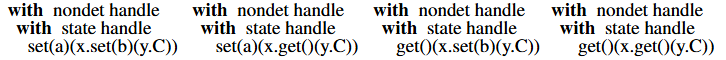
\includegraphics[width=1\textwidth]{localStateHandlerComp.png}

\caption{Standard state laws remain valid under local state, as all state operations are resolved within each branch rather than between them.}
\label{fig:local-state-laws}
\end{figure}


\subsubsection{Impermanence} 
\begin{tcolorbox}[colback=gray!10, colframe=gray!60, sharp corners, boxrule=0.5pt, title={POSIX Base Specifications, Issue 7, p.554}]
Memory mappings that were created in the process shall be unmapped before the process
 is destroyed.
 \end{tcolorbox}
 
The specification above advises that a process's local state should be lost when the process is destroyed. Whilst there is no direct correspondence to the properties for \textit{backtrackable state} shown in Tang and Schrijvers paper, an anology with the \lstinline{fail} operation $\varnothing$ can be drawn. The identities below show how state is lost after failure: 

\[
\textbf{put-right-identity}: \quad \texttt{put}\;s \gg \varnothing = \varnothing
\]
\vspace{-1em}
\[
\textbf{get-right-identity}: \quad \texttt{get}\; \gg \varnothing = \varnothing
\]

The placement of the state handler inside the nondeterminism handler ensures that state is scoped to each branch individually and when a computation returns, its state is no longer stored. The return clause  simply returns a value and does not resume the continuation, thereby losing all variable bindings and its associated state. 

\vspace{1em}
{\large{\textbf{Proof of Idempotence of return and local state}}}

\normalsize



\begin{longtable}{@{}l@{}}
\textbf{with } nondet handle \\
\quad \textbf{with } state handle \\
\quad\quad set(a)(x. return 0) \, ++ \, set(b)(y. return 0) \\

\quad$\equiv$ (11) \\

\textbf{with } nondet handle \\
\quad fun \_ $\rightarrow$ (k())s \ [a/s,\ fun y $\rightarrow$ \textbf{with } state handle return 0]\\
\quad\quad ++ \\
\quad fun \_ $\rightarrow$ (k())s \ [b/s,\ fun y $\rightarrow$ \textbf{with } state handle return 0] 
\quad$\equiv$ (subst) \\
\textbf{with } nondet handle \\
\quad fun \_ $\rightarrow$ (fun y $\rightarrow$ \textbf{with } state handle return 0)() \ a \\
\quad\quad ++ \\
\quad fun \_ $\rightarrow$ (fun y $\rightarrow$ \textbf{with } state handle return 0)() \ b \\
\quad$\equiv$ (8) \\
\textbf{with } nondet handle \\
\quad fun \_ $\rightarrow$ (\textbf{with } state handle return 0) \ a \\
\quad ++ \\
\quad fun \_ $\rightarrow$ (\textbf{with } state handle return 0) \ b \\
\quad$\equiv$ (10) \\
\textbf{with } nondet handle \\
\quad fun \_ $\rightarrow$ 0 \ a \quad ++ \quad fun \_ $\rightarrow$ 0 \ b \\
\quad$\equiv$ (apply) \\
\textbf{with } nondet handle \\
\quad 0 ++ 0 \\
\end{longtable}


\subsubsection{State Inheritance} 
\begin{tcolorbox}[colback=gray!10, colframe=gray!60, sharp corners, boxrule=0.5pt, title={POSIX Base Specifications, Issue 7, p.897}]
Memory mappings created in the parent shall be retained in the child process
\end{tcolorbox}
The specification above advises that when a process forks the state in the parent should be copied for the child. This ensures that both processes start from an identical state from which they may then proceed independently.

Tang and Schrijvers \cite{tang2025high} show how their \textit{backtrackable state} Monad displays state distribution across nondeterministic choice:


\begin{figure}[H]  % Use [H] to force exact placement, or [htbp] for flexible
  \centering
  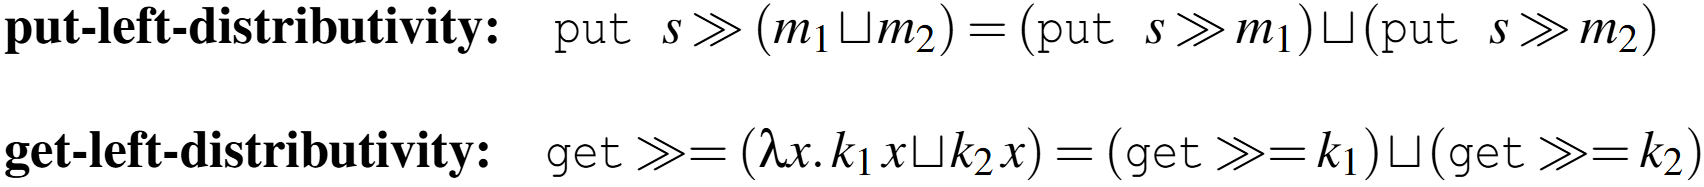
\includegraphics[width=1\textwidth]{distributivity.png}  % Adjust width & filename
  
\end{figure}

In line with the above properties, I can demonstrate that my handlers allow state operations to distribute over forking, following the inheritance functionality prescribed in the Unix specification. 


{\large{\textbf{Proof - \textit{Get} Distributing Over \textit{Fork}}}}







\subsection{Unix Specifications: Global State }

\begin{tcolorbox}[colback=gray!10, colframe=gray!60, sharp corners, boxrule=0.5pt, title={POSIX Base Specifications, Issue 7, p.2316}]
 This volume of POSIX.1-2008 does not specify the behaviour of concurrent writes to a regular file |
 from multiple threads, except that each write is atomic (see Section 2.9.7, onpage 522). |
 Applications should use some form of concurrency control.
\end{tcolorbox}

The term \textit{global state} refers to any memory or system resources that are shared across processes and includes the file system and other kernel-managed structures that persist independently of any single process. Since \textit{state} is potentially modifiable by other concurrently running processes, a change made in one process can affect the behaviour of others. The Unix specifications acknowledges this concurrency problem and deals with it by delegating it to the application level. A topic that will be discussed in more detail later in this chapter.

Since execution ordering depends on the dynamic runtime state of the scheduler, algebraic reasoning about global state, it is inapplicable in this scenario. 

Tang and Schrijvers also encounter this problem when trying to represent global state using monads. They point out that while global state and nondeterminism can each be given a monadic structure, their composition cannot be modelled as a monad in the usual way. The problem is that state updates persist across nondeterministic branches, which breaks two of the key monad laws, associativity and identity. The composition of \textit{nondeterminism} and \textit{state} fails to maintain the property of right-distributivity of \textit{nondeterminism}.


Tang and Schrijver's describe one possible global state law,  the \textit{put-or} law. This law is valid in an \textcolor{red}{operational model} where state updates are evaluated from left to right.

\[
\textbf{put-or:} \quad (put\ s \gg m) \oplus n = put\ s \gg (m \oplus n) 
\]

However, this another example of the equational theory being too strong to hold in a practical implementation: in Unix systems, the order in which a scheduler's policy will run the processes cannot be assumed.


The limits of algebraic reasoning for global state evaluation are shown below. In this example a computation is evaluated until it can not be evaluated any further, because after this point the scheduler must determine the execution order.

\vspace{1em}
{\large \textbf{Example of Global State Evaluation}}
\begin{longtable}{@{}l@{}}
\textbf{with } state \textbf{ handle} \\
\quad \textbf{with } nondet \textbf{ handle} \\
\quad\quad Fork()(p.\textbf{if } p \textbf{ then } set(x)(a.C\textsubscript{1}) \textbf{ else } set(y)(b.C\textsubscript{2})) \\
\quad$\equiv$ (11) \\
\\
\textbf{with } state \textbf{ handle} \\
\quad \textbf{resume } True \text{ ++ } \textbf{resume } False \\
\quad [()/v,\ \text{fun } r $\rightarrow$ \textbf{with } nondet \textbf{ handle if } r \textbf{ then } set(x)(a.C1) \textbf{ else } set(y)(b.C2)] \\
\\
\quad$\equiv$ (\text{subst}) \\
\textbf{with } state \textbf{ handle} \\
\quad fun r $\rightarrow$ \textbf{with } nondet \textbf{ handle if } r \textbf{ then } set(x)(a.C1) \textbf{ else } set(y)(b.C2)\ True \\
\quad ++ \\
\quad fun r $\rightarrow$ \textbf{with } nondet \textbf{ handle if } r \textbf{ then } set(x)(a.C1) \textbf{ else } set(y)(b.C2)\ False \\
\\
\quad$\equiv$ (8) \\
\textbf{with } state \textbf{ handle} \\
\quad \textbf{with } nondet \textbf{ handle if } True \textbf{ then } set(x)(a.C1) \textbf{ else } set(y)(b.C2) \\
\quad ++ \\
\quad \textbf{with } nondet \textbf{ handle if } False \textbf{ then } set(x)(a.C1) \textbf{ else } set(y)(b.C2) \\
\\
\quad$\equiv$ (5,6) \\
\textbf{with } state \textbf{ handle} \\
\quad \textbf{with } nondet \textbf{ handle } set(x)(a.C1) \\
\quad ++ \\
\quad \textbf{with } nondet \textbf{ handle } set(y)(b.C2) \\
\\
\quad$\equiv$ (12) \\
\textbf{with } state \textbf{ handle} \\
\quad set(x)(a.\textbf{with } nondet \textbf{ handle } C1) \\
\quad ++ \\
\quad set(y)(b.\textbf{with } nondet \textbf{ handle } C2) \\
\end{longtable}


It will be seen that this creates a nondeterministic outcome, as the order in which the scheduler chooses to run these branches will affect the final state of the system. 




\section{Properties of Processes}

Having clarified the algebraic properties of individual effects and the properties of global and local scope depending on handler ordering, we now look at what properties processes maintain when combining  non determinism, global state, local state.

In this section, we also introduce the exit effect, a non-resumable control operation that disrupts sequencing, and explore how its interaction with other handlers further affects compositional reasoning.


\subsubsection*{Local State Breaks Associativity}

In the purely nondeterministic setting, forking is associative, i.e. the grouping/nesting does not affect its semantics. However in the 

\textcolor{red}{According to most equational theories nondeterminism is supposed to be associative in }

\begin{table}[H]
\centering
\begin{tabular}{p{0.45\textwidth} c p{0.45\textwidth}}
\begin{lstlisting}
if Fork(){
    // A
    if Fork(){
        // A continued
        pass
    }
    else{
        // C
    }
}
else{
    set("B")
}
\end{lstlisting}
&
&
\begin{lstlisting}
if Fork(){
    A
} 
else{
    // B
    set("B");
    if Fork(){
        // B continued
        pass
    }
    else{
        // C
        C
    }
}
\end{lstlisting}
\end{tabular}
\end{table}
\vspace{-2em}


\subsubsection*{Local State Full Distributivity}
Whilst left distributivity does not hold in general, it does hold in the special case of idempotent effects, where repeated applications of R are equivalent to applying it once. As right distributivity holds trivially through algebraicity of sequencing Local State is fully distributive 

\vspace{-2em}
\begin{table}[H]
\centering
\begin{tabular}{p{0.45\textwidth} c p{0.45\textwidth}}
\begin{lstlisting}
set(x);
if Fork(){
    P;
}
else{
    Q;
}
\end{lstlisting}
&
&
\begin{lstlisting}
if Fork(){
    set(x); 
    P;
}
else{ 
    set(x); 
    Q;
}
\end{lstlisting}
\end{tabular}
\end{table}
\vspace{-2em}


\subsection{Summary of Properties Under Composition}


\section{Exceptions}
Processes can terminate successfully by running to completion, or they can terminate by performing an exit system call. The exit call takes a numeric argument indicating the exit status of the process. Unlike other operations exit does not allow for continuation, it discards the remaining computation and terminates execution immediately.

Exceptions disrupt all of the algebraic properties that held before hand, these properties now only hold on the assumption that there is no exception in their scope. Exceptions only hold one property, that any code that succeeds them is semantically irrelevant.


\begin{figure}[H]
\centering

% Effect signature
\effectDef{\textbf{Status}}{\text{Exit : Int} \rightarrow 0}

\vspace{-1em}

% Handler implementation
\[
\mathrm{status} \;\overset{\mathrm{def}}{=}\;
\mathrm{handler} \;\left\{
\begin{array}{ll}
  \mathrm{\textbf{return}\:\_} & \mapsto 0 \\[0.5ex]
  \langle\!\langle \mathrm{Exit} \langle n\rangle\rangle & \mapsto n \\[0.5ex]
\end{array}
\right\}
\]

\caption{Effect signature and handler implementation of exceptions via the \textbf{Status} effect.}
\label{fig:status-handler}
\end{figure}

\subsection*{Absorption}

The absorption property states that once an exit operation is called within a computation, any further computation is irrelevant. The following formalises the property that, whatever comes after the exit, does not affect the behaviour of the program:

\equivalenceStatement{status}{Exit (n)(y.C)}{status}{Exit(n)(y.D)}

Because Exit n returns type 0, the uninhabited type, it cannot yield a result. To embed it in a computation expecting a value of type $\alpha$, we use the absurd function to coerce from the empty type to $\alpha$. This reflects that any code after Exit n is unreachable, and ensures the expression remains well-typed.

\[
\mathrm{exit\:n} \;\overset{\mathrm{def}}{=}\;
\mathrm{handler} \;\left\{
\begin{array}{l}
  \text{absurd\:(\textbf{do}\:Exit\:n)} \quad\\[0.5ex]

\end{array}
\right\}
\]

\underline{Left Hand Side}

\[
\begin{array}{l}
\quad\equiv\quad (\text{subst}) \\[5pt]
\text{absurd (do Exit } n) (y. C) \\[5pt]
\quad\equiv\quad (11) \\[5pt]
v [n/v, \text{fun } y \rightarrow \text{\textbf{with} status \textbf{handle} } C/k] \\[5pt]
\quad\equiv\quad (\text{subst}) \\[5pt]
n
\end{array}
\]

\underline{Right Hand Side}

\[
\begin{array}{l}
\quad\equiv\quad (11) \\[5pt]
\text{absurd (do Exit } n) (y. D) \\[5pt]
\quad\equiv\quad (11) \\[5pt]
v [n/v, \text{fun } y \rightarrow \text{\textbf{with} status \textbf{handle} } D/k] \\[5pt]
\quad\equiv\quad (\text{subst}) \\[5pt]
n
\end{array}
\]


\section{Process Synchronisation}
So far we have introduced a basic time-sharing, using interrupts and the scheduler, that allows the interleaving of process execution. However, as mentioned before, the way that processes are interleaved is non-deterministic, in other words processes don't know the order in which the will be executed. 

This is a problem because, as we have demonstrated, many of our effects are non-commutative meaning that the order of execution is important for correctness. This creates what is known as a "race condition", A race condition arises when the correctness of a program depends on the nondeterministic interleaving of concurrent operations on shared state. Without explicit synchronisation, the outcome is unpredictable and may differ across runs, making correct behaviour accidental rather than guaranteed.

Currently the only way to guarantee execution order is to execute all the steps, in the same process, sequentially with no interrupts which defeats the point of our time sharing system as no interleaving is possible in this time, which blocks the other processes.

To introduce flexibility around process interleaving whilst maintaining guarantees about execution ordering we introduced two features
\begin{itemize}
    \item \lstinline{Wait} \textbf{system calls: } This allows a parent to suspend execution until its child process (identified by its process id) has finished executing. Think of this as introducing a causal dependency, the parent can only when the child finishes.
    \item \textbf{Mutexes: } This a process to lock a resource, meaning that whilst the process holds this lock, no other process can alter this resource. This guarantees that between interrupts other processes don't alter the resource, which could potentially lead to file corruption. 
\end{itemize}

Combining these two properties by;
\begin{enumerate}
    \item Locking the resource, to prevent other processes simultaneously writing to (and thereby corrupting) our resource
    \item Splitting up the responsibility for writes between its children, and waiting in order for them to complete
    \item Unlocking the resource to allow other processes to access it
\end{enumerate}

we can provide partial ordering guarantees about write safety whilst still allowing for concurrency.


Reasoning about the scheduler is very difficult because it introduces non-determinism into our system. Unlike the algebraic effects, which have clear equational rules, the behaviour of the scheduler depends on the runtime state of the process queue and the particular order in which processes are resumed. 

Unfortunately reasoning about the scheduler has long been difficult to reason about \cite{}. As noted in \textit{The Logic and Handling of Algebraic Effects}, recursive definitions over both parameters are not primitively recursive. There is no clear "smaller" structure to descend into as neither parameter is fixed while the other reduces. This breaks traditional inductive reasoning and requires more complex mutual or nested inductions, which are notoriously difficult to manage algebraically.






\section{Reasoning Conclusions}

In this section we have demonstrated how to use algebraic equivalences to reason about effect handlers. We first examined different models of state depending on how we composed the nondeterminism and state handlers, which corresponded to global file system state and process local state. We verified that each of these models fulfilled the properties that Unix expected them to have. 

We then went on to reason about other interesting properties that the equivalences allowed us to show. This helped to verify that certain program transformations are valid and allowed us to simplify our code. 

We also discovered that many of the rules that held in an isolated setting break down under composition. 

It is very difficult to reason about any properties which rely on the scheduler. This makes reasoning about any forms of process synchronsiation or interprocess communication very difficult to do. Unfortunately effects like \lstinline{Wait} or \lstinline{Acquire} \lstinline{Release} which introduce partial order semantics can't be easily reasoned about using our equivalences as they depend upon the dynamic execution state of our system.

\chapter{Conclusions}

\section{Unix Implementation in Koka}
We have successfully realised the "Toy Unix" system described in Hillerström's paper, we provided implementations for exception handling, a basic IO scheme, user functionality, a basic serial file system, piping and two methods of process scheduling. We achieved the goal we set out to do namely, to show that we can implement a simulation of Unix, tackling the complex problems this presents, in a concise and modular way.

\subsection*{Future Work}
Implementing the process synchronisation features described in the previous chapter would provide vital functionality to our Unix system. Currently, if the system wants to perform writes in order, it can't do any interleaving, meaning that all writes are blocking defeating the purpose of a time-sharing system. Mutexes would provide a simple way to guarantee that resources can't be tampered with.

\section{Reasoning}
We successfully verified that our implementation of Unix follows the rules expected of it according to the Unix Specifications. We quickly ran into problems when trying to reason about anything which was not directly related to code structure, the dynamic state of the scheduler prevented us doing any reasoning about synchronisation or IPC.
\subsection*{Future}
Further reasoning about partial ordering of effectful operations using Waits and Mutexes. We could also implement a model of Local File Descriptor tables for processes and a global Open File Table. This would open up reasoning about sharing and isolation of state and how this aids modularity and functionality.  

% \bibliographystyle{plain}
\bibliographystyle{plain}
\bibliography{mybibfile}


% You may delete everything from \appendix up to \end{document} if you don't need it.
\appendix

\chapter{Single-cell state proofs} 

\section{Simplified State} \label{full-simplified-single-cell-state-proof}

\subsubsection*{Idempotence of Set}
Performing consecutive \lstinline{set} operations retains only the final update, as each invocation completely overwrites the current state:
\[
\begin{aligned}
    &\mathsf{\textbf{with}} \; \mathsf{state} \; \mathsf{\textbf{handle}} \\
    &\quad \operatorname{set} \; a \; (x. \operatorname{set} \; b \; (y. C)) \\
    &\equiv \\
    &\mathsf{\textbf{with}} \; \mathsf{state} \; \mathsf{\textbf{handle}} \\
    &\quad \operatorname{set} \; b \; (y. C)
\end{aligned}
\]

\underline{Left Hand Side}

\[ 
\begin{array}{l}
\quad\equiv\quad (11) \\[5pt]
\text{fun }\_ \rightarrow (k\ ())\ s\ [a/s,\ \text{fun } x \rightarrow \text{\textbf{with} state \textbf{handle} } set(b)(y.C)/k] \\[5pt]
\quad\equiv\quad (\text{subst}) \\[5pt]
\text{fun }\_ \rightarrow ((\text{fun } x \rightarrow \text{\textbf{with} state \textbf{handle} } set(b)(y.C))\ ())\ a \\[5pt]
\quad\equiv\quad (8) \\[5pt]
\text{fun }\_ \rightarrow (\text{\textbf{with} state \textbf{handle} } set(b)(y.C))\ a \\[5pt]
\quad\equiv\quad (11) \\[5pt]
\text{fun }\_ \rightarrow (\text{fun }\_ \rightarrow (k\ ())\ s\ [b/s, \text{fun } y \rightarrow \text{\textbf{with} state \textbf{handle} } C/k])\ a \\[5pt]
\quad\equiv\quad (\text{subst}) \\[5pt]
\text{fun }\_ \rightarrow (\text{fun }\_ \rightarrow (\text{fun } y \rightarrow \text{\textbf{with} state \textbf{handle} } C)\ ())\ b)\ a \\[5pt]
\quad\equiv\quad (8) \\[5pt]
\text{fun }\_ \rightarrow (\text{fun }\_ \rightarrow (\text{\textbf{with} state \textbf{handle} } C)\ b)\ a \\[5pt]
\quad\equiv\quad (\text{application}) \\[5pt]
\text{fun }\_ \rightarrow (\text{\textbf{with} state \textbf{handle} } C)\ b
\end{array}
\]

\underline{Right Hand Side}
\[ 
\begin{array}{l}
\quad\equiv\quad (11) \\[5pt]
\text{fun }\_ \rightarrow (k\ ())\ s\ [b/s, \text{fun } y \rightarrow \text{\textbf{with} state \textbf{handle} } C/k] \\[5pt]
\quad\equiv\quad (\text{subst}) \\[5pt]
\text{fun }\_ \rightarrow ((\text{fun } y \rightarrow \text{\textbf{with} state \textbf{handle} } C)\ ())\ b \\[5pt]
\quad\equiv\quad (8) \\[5pt]
\text{fun }\_ \rightarrow (\text{\textbf{with} state \textbf{handle} } C)\ b
\end{array}
\]

LHS $\equiv$ RHS

\subsubsection*{Idempotence of Get}
Reading the state multiple times without an intervening \lstinline{set} yields the same result each time. Repeating a get operation without modifying the state in between has no observable effect on the computation.


\[
\begin{aligned}
    &\mathsf{\textbf{with}} \; \mathsf{state} \; \mathsf{\textbf{handle}} \\
    &\quad \operatorname{get}() \left( \mathsf{x.get}() \left( y.C \right) \right) \\
    &\equiv \\
    &\mathsf{\textbf{with}} \; \mathsf{state} \; \mathsf{\textbf{handle}} \\
    &\quad \operatorname{get}() \left( x.C[x/y] \right)
\end{aligned}
\]
\underline{Left Hand Side}

\[ 
\begin{array}{l}
\quad\equiv\quad (11) \\[5pt]
\text{fun } s \rightarrow (k\ s)\ s\ [()/v, \text{fun } x \rightarrow \text{\textbf{with} state \textbf{handle} } get()(y.C)/k] \\[5pt]
\quad\equiv\quad (\text{subst}) \\[5pt]
\text{fun } s \rightarrow ((\text{fun } x \rightarrow \text{\textbf{with} state \textbf{handle} } get()(y.C))\ s)\ s \\[5pt]
\quad\equiv\quad (8) \\[5pt]
\text{fun } s \rightarrow (\text{\textbf{with} state \textbf{handle} } get()(y.C[s/x]))\ s \\[5pt]
\quad\equiv\quad (11) \\[5pt]
\text{fun } s \rightarrow ((\text{fun } s'\rightarrow (k\ s')\ s')\ [()/v, \text{fun } y\rightarrow \text{\textbf{with} state \textbf{handle}}/k])\ s \\[5pt]
\quad\equiv\quad (\text{subst}) \\[5pt]
\text{fun } s \rightarrow ((\text{fun } s' \rightarrow (( \text{fun } y \rightarrow \text{\textbf{with} state \textbf{handle} } C[s/x])\ s')\ s')\ s \\[5pt]
\quad\equiv\quad (8) \\[5pt]
\text{fun } s \rightarrow (\text{fun } s' \rightarrow (\text{\textbf{with} state \textbf{handle} } C[s/x][s'/y]s')) \\[5pt]
\quad\equiv\quad (8) \\[5pt]
\text{fun } s \rightarrow (\text{\textbf{with} state \textbf{handle} } C[s/x][s/y])\ s
\end{array}
\]



\underline{Right Hand Side}

\[ 
\begin{array}{l}
\quad\equiv\quad (11) \\[5pt]
\text{fun } s \rightarrow (k\ s)\ s\ [()/v, C[x/y]] \\[5pt]
\quad\equiv\quad (\text{subst}) \\[5pt]
\text{fun } s \rightarrow ((\text{fun } x \rightarrow \text{\textbf{with} state \textbf{handle} } C[x/y])) \\[5pt]
\quad\equiv\quad (8) \\[5pt]
\text{fun } s \rightarrow (\text{\textbf{with} state \textbf{handle} } C[x/y][s/x])\ s
\end{array}
\]

LHS $\equiv$ RHS



\subsubsection*{Set-Then-Get}
Reading the state immediately after setting it yields the value that was just written. This property ensures that state updates are immediately observable.
\[
\begin{aligned}
    &\mathsf{\textbf{with}} \; \mathsf{state} \; \mathsf{\textbf{handle}} \\
    &\quad \operatorname{set} \; a \; (x. \operatorname{get}() \; (y. C)) \\
    &\equiv \\
    &\mathsf{\textbf{with}} \; \mathsf{state} \; \mathsf{\textbf{handle}} \\
    &\quad \operatorname{set} \; a \; (x. C[a/x])
\end{aligned}
\]

\underline{Left Hand Side}
\[ 
\begin{array}{l}
\quad\equiv\quad (11) \\[5pt]
\text{fun }\_ \rightarrow (k\ ())\ s\ [a/s, \text{fun } x \rightarrow \text{\textbf{with} state \textbf{handle} } get() (y. C)/k] \\[5pt]
\quad\equiv\quad (\text{subst}) \\[5pt]
\text{fun }\_ \rightarrow ((\text{fun } x \rightarrow \text{\textbf{with} state \textbf{handle} } get() (y. C)) ())\ a \\[5pt]
\quad\equiv\quad (8) \\[5pt]
\text{fun }\_ \rightarrow (\text{\textbf{with} state \textbf{handle} } get() (y. C))\ a \\[5pt]
\quad\equiv\quad (11) \\[5pt]
\text{fun }\_ \rightarrow (\text{fun } s' \rightarrow  (k\ s')\ s' [()/s, \text{fun } y \rightarrow \text{\textbf{with} state \textbf{handle} } C / k])\ a \\[5pt]
\quad\equiv\quad (\text{subst}) \\[5pt]
\text{fun }\_ \rightarrow ((\text{fun } s' \rightarrow ((\text{fun } y \rightarrow \text{\textbf{with} state \textbf{handle} } C)\ s' )\ s')\ a \\[5pt]
\quad\equiv\quad (\text{application}) \\[5pt]
\text{fun }\_ \rightarrow ((\text{fun } y \rightarrow \text{\textbf{with} state \textbf{handle} } C)\ a )\ a \\[5pt]
\quad\equiv\quad (8) \\[5pt]
\text{fun }\_ \rightarrow (\text{\textbf{with} state \textbf{handle} } C[a/y])\ a
\end{array}
\]

\underline{Right Hand Side}
\[ 
\begin{array}{l}
\quad\equiv\quad (11) \\[5pt]
\text{fun }\_ \rightarrow (k\ ())\ s\ [a/s, \text{fun } x \rightarrow \text{\textbf{with} state \textbf{handle} } C[a/y]/k] \\[5pt]
\quad\equiv\quad (\text{subst}) \\[5pt]
\text{fun }\_ \rightarrow ((\text{fun } x \rightarrow \text{\textbf{with} state \textbf{handle} } C[a/y]) ())\ a \\[5pt]
\quad\equiv\quad (8) \\[5pt]
\text{fun }\_ \rightarrow (\text{\textbf{with} state \textbf{handle} } C[a/y])\ a
\end{array}
\]



\subsubsection*{Get-Then-Set}
A \lstinline{get} followed by a \lstinline{set}, updates the state with a new value whilst preserving the former state value by binding it in the continuation. 


\[
\begin{aligned}
    &\mathsf{\textbf{with}} \; \mathsf{state} \; \mathsf{\textbf{handle}} \\
    &\quad \operatorname{get}() \left( x. \operatorname{set} \; a \; (y. C) \right) \\
    &\equiv \\
    &\mathsf{\textbf{with}} \; \mathsf{state} \; \mathsf{\textbf{handle}} \\
    &\quad \operatorname{set} \; a \; (y. C[s/x])
\end{aligned}
\]

\underline{Left Hand Side}
\[ 
\begin{array}{l}
\quad\equiv\quad (11) \\[5pt]
\text{fun } s \rightarrow (k\ s)\ s\ [()/v, \text{fun } x \rightarrow \text{\textbf{with} state \textbf{handle} } set(a)(y.C)/k] \\[5pt]
\quad\equiv\quad (\text{subst}) \\[5pt]
\text{fun } s \rightarrow ((\text{fun } x \rightarrow \text{\textbf{with} state \textbf{handle} } set(a)(y.C))\ s)\ s \\[5pt]
\quad\equiv\quad (8) \\[5pt]
\text{fun } s \rightarrow (\text{\textbf{with} state \textbf{handle} } set(a)(y.C[s/x]))\ s \\[5pt]
\quad\equiv\quad (11) \\[5pt]
\text{fun } s \rightarrow ((\text{fun } \_ \rightarrow (k\ ())\ s')[a/s', \text{fun } y \rightarrow \text{\textbf{with} state \textbf{handle} } C[s/x]/k])\ s' \\[5pt]
\quad\equiv\quad (\text{subst}) \\[5pt]
\text{fun } s \rightarrow (\text{fun } \_ \rightarrow (\text{\textbf{with} state \textbf{handle} } C[s/x]) ())\ a \\[5pt]
\quad\equiv\quad (8) \\[5pt]
\text{fun } s \rightarrow (\text{\textbf{with} state \textbf{handle} } C[s/x])\ a
\end{array}
\]


\underline{Right Hand Side}
\[ 
\begin{array}{l}
\quad\equiv\quad (11) \\[5pt]
\text{fun }\_ \rightarrow (k\ ())\ s\ [a/s, \text{fun } y \rightarrow \text{\textbf{with} state \textbf{handle} } C[s/x]/k] \\[5pt]
\quad\equiv\quad (\text{subst}) \\[5pt]
\text{fun }\_ \rightarrow (\text{fun } y \rightarrow \text{\textbf{with} state \textbf{handle} } C[s/x]) ()\ a \\[5pt]
\quad\equiv\quad (8) \\[5pt]
\text{fun }\_ \rightarrow (\text{\textbf{with} state \textbf{handle} } C[s/x]\ a)
\end{array}
\]
LHS $\equiv$ RHS

\section{Environment Variable Proofs} \label{environment-variable-proofs}

\chapter{Participants' information sheet}

If you had human participants, include key information that they were given in
an appendix, and point to it from the ethics declaration.

\chapter{Participants' consent form}

If you had human participants, include information about how consent was
gathered in an appendix, and point to it from the ethics declaration.
This information is often a copy of a consent form.


\end{document}
